\chapter{Grundlagen}
In diesem Kapitel sollen die für das weitere Verständnis notwendigen theoretischen Grundlagen erläutert werden. Dazu gehört zunächst der Aufbau des Netzwerks in einem Fahrzeug. Des Weiteren werden relevante Grundlagen der Cyber Security erklärt.

\section{Automotive Networking}
Im Inneren von Autos befinden sich heutzutage eine Vielzahl elektronischer Systeme, von denen jedes mit benachbarten Komponenten kommunizieren kann. Die einzelnen elektronischen Systeme werden als \acp{ECU} bezeichnet. Moderne Autos enthalten in der Regel über 50 verschiedene \acsp{ECU} \cite[vgl.][6]{Miller.2013}. Da diese Kontrolleinheiten zum Teil lebensentscheidende Aufgaben übernehmen, muss die Kommunikation zwischen den Einheiten möglichst in Echtzeit erfolgen. \\

\begin{figure}[H]
\centering
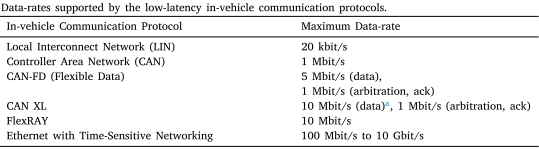
\includegraphics[width=\textwidth]{communication-protocols}
\label{fig:communication-protocols}
\caption{Verschiedene Kommunikationsprotokolle in Automobil-Netzwerken}
\quelle{\cite[2]{MohammadAshjaei.2021}}
\end{figure}

Für die Vernetzung der \acsp{ECU} kommen verschiedene Technologien zum Einsatz (siehe Abbildung \ref{fig:communication-protocols}). Die relevantesten davon werden im Folgenden genauer erläutert. Die wichtigste  davon ist im Automotive-Bereich der sogenannte \acs{CAN}-Standard.

\subsection{Controller Area Network}
Die elektronischen Kontrolleinheiten eines Autos sind typischerweise über einen oder mehrere Busse, die auf dem \ac{CAN}-Standard basieren, miteinander verbunden. Hierbei kommunizieren die \acsp{ECU} über \acs{CAN}-Pakete. Diese werden an alle Komponenten gesendet, welche dann jeweils basierend auf dem Inhalt entscheiden, ob das Paket für sie bestimmt ist oder nicht. Eine Identifikation der Quelle oder Authentisierung gibt es in diesem Standard nicht. \cite[vgl.][7]{Miller.2013} \\
Generell wird meistens zwischen High Speed \acs{CAN} und Low Speed \acs{CAN} unterschieden. High Speed \acs{CAN} wird eingesetzt, wenn bei der Übertragung hohe Geschwindigkeit benötigt wird, beispielsweise bei sicherheitskritischen Anwendungsfällen. Außerdem wird bietet sich die Verwendung von High Speed \acs{CAN} bei der Übertragung von großen Datenmengen an.
In Abbildung \ref{fig:canbus-ford2010} ist das \acs{CAN}-Netzwerk eines 2010 Ford Escape dargestellt. Das abgebildete Netzwerk verfügt über zwei Busse, einen medium speed (MS) und einen high speed (HS) \acs{CAN}-Bus. Beide Busse enden hier im \ac{DLC} (siehe Kapitel \ref{OBD-II}).
In Automotive Netzwerken lassen sich zwei Arten von \acs{CAN}-Paketen finden: normale \acs{CAN}-Pakete und diagnostische \acs{CAN}-Pakete. 

\begin{figure}[H]
\centering
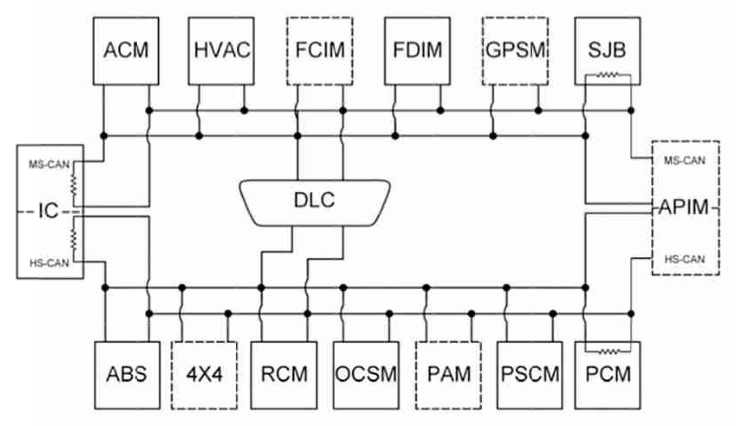
\includegraphics[width=0.7\textwidth]{Miller_canbus-ford2010}
\label{fig:canbus-ford2010}
\caption{Beispiel des \acs{CAN}-Netzwerks eines 2010 Ford Escape}
\quelle{\cite[19]{Miller.2013}}
\end{figure}

\subsubsection{Normale \acs{CAN}-Pakete}
Normale Pakete werden von \acsp{ECU} gesendet und können entweder Informationen oder Befehle enthalten. Typischerweise werden sie alle Millisekunden gesendet. Auf Anwendungsebene enthalten die \acs{CAN}-Pakete einen Identifier, die zu übertragenden Daten und manchmal noch eine Prüfsumme, um sicherzustellen, dass das Paket korrekt übertragen wurde. Der Identifier gibt sowohl an, für welche \acsp{ECU} das Paket bestimmt ist, als auch, welche Priorität das Paket hat. \cite[vgl.][9]{Miller.2013}\\
Das Format einer \acs{CAN}-Botschaft ist in Abbildung \ref{fig:CanBotschaft} dargestellt. Es besteht aus folgenden Bestandteilen:
\subparagraph{Header} CAN ist ein Broadcast-System, bei dem jeder Sender seine Botschaften mit einem eindeutigen Message Identifier markiert.
\subparagraph{Message Identifier} Der Message Identifier kennzeichnet eine Botschaft und dient zur eindeutigen Identifizierung. Er kann entweder 11 Bit (CAN 2.0A) oder 29 Bit (CAN 2.0B) lang sein und enthält zusätzlich 1 bis 3 Steuerbits.
\subparagraph{Control Bits} Die Steuerbits im Control-Feld umfassen den Data Length Code (DLC), der die Anzahl der übertragenen Nutzdatenbytes angibt, sowie eine 15-Bit-Prüfsumme, auch genannt Cyclic Redundancy Check (CRC) zur Fehlererkennung.
\subparagraph{Payload} Die Nutzdaten (Payload) einer Botschaft können zwischen 0 und 8 Datenbytes umfassen.
\subparagraph{Acknowledge und End of Frame} Die CAN-Controller der Empfänger senden eine positive Empfangsbestätigung oder eine Fehlermeldung (Error Frame) innerhalb des Acknowledge und End of Frame Felds.
\subparagraph{Stuffing Bits} Stuffing Bits werden verwendet, um den Bittaktgenerator von Empfängern zu synchronisieren. Sie werden eingefügt, um sicherzustellen, dass nicht mehr als fünf aufeinanderfolgende Bits denselben Wert haben. \cite[61\psqq]{Zimmermann.2014}

\begin{figure}[h]
\centering
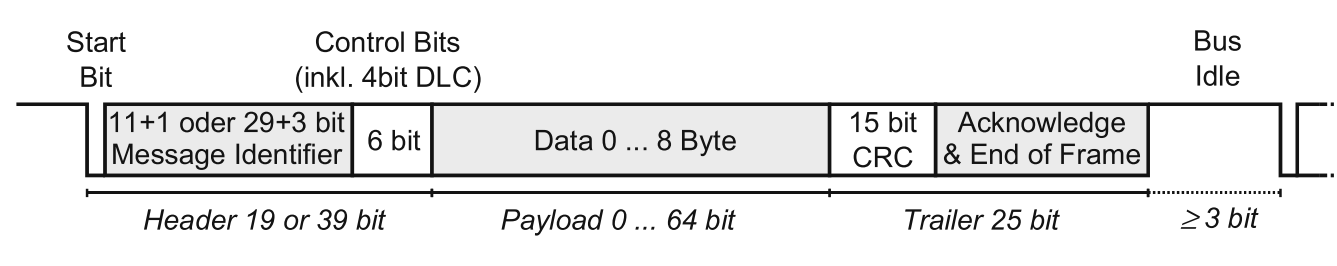
\includegraphics[width=\textwidth]{Zimmermann_CanBotschaft}
\label{fig:CanBotschaft}
\caption{Format einer \acs{CAN}-Botschaft}
\quelle{\cite[61]{Zimmermann.2014}}
\end{figure}


\subsubsection{Diagnostische \acs{CAN}-Pakete}
Diagnostische Pakete tauchen während des normalen Betriebs des Autos im Normalfall nicht auf. Sie werden von Diagnose-Werkzeugen gesendet, die beispielsweise von Mechanikern genutzt werden um mit den \acsp{ECU} im Auto zu kommunizieren. So können Mängel und Fehlfunktionen entdeckt oder andere Informationen gewonnen werden. Das Format von diagnostischen \acs{CAN}-Paketen ähnelt dem von normalen Paketen, erfolgt jedoch meist nach strengeren Konventionen. Standards hierfür sind zum Beispiel ISO-TP, ISO 14229 und ISO 14230. \cite[vgl.][10]{Miller.2013}

\subsection{Local Interconnect Network}
Ein weiteres relevantes Protokoll im Automotive Bereich ist das \ac{LIN} Protokoll. Es wurde 1998 in Zusammenarbeit von Audi, BMW, DaimlerChrysler, Volvo, Volkswagen, VCT und Motorola entwickelt mit dem Ziel, ein möglichst kosteneffizientes Kommunikationsprotokoll zu schaffen \cite[57]{Fijalkowski.2011}.
Das \acs{LIN}-Protokoll basiert auf dem Serial Connections Interface Datenformat und ist in einer Single Master/Multiple Slaves Architektur aufgebaut. Das bedeutet, dass eine elektronische Kontrolleinheit als Masterknoten fungiert und andere elektronische Slave-Einheiten miteinander verbindet.


\subsubsection{Aufbau}
Nachrichtenpakete bestehen im \acs{LIN}-Standard aus einem Header und einem Data Frame. Der Header enthält einen Synchronisation Break, ein Synchronisation Byte und einen Message Identifier. Die ersten beiden Bestandteile sind für die Nachrichtensynchronisierung notwendig. Der Identifier wird benötigt, damit Knoten erkennen können, ob eine Nachricht für sie bestimmt ist. Der Data Frame ist nach dem 8N1-Schema aufgebaut. Das bedeutet, dass jedes Paket ein Startbit, acht Datenbits, kein Paritätsbit und ein Stopbit besitzt. \cite[58]{Fijalkowski.2011} \\
Im \acs{LIN}-Standard sind drei Arten von Kommunikation erlaubt.
\begin{enumerate}
\item Master to Slave, beziehungsweise Master to Multiple Slaves
\item Slave to Master
\item Slave to Slave
\end{enumerate}
Die Slaves können somit auch untereinander ohne Beiteiligung des Masters kommunizieren. \cite[59]{Fijalkowski.2011}

\subsubsection{Anwendung}
\ac{LIN} zeichnet sich wie oben erwähnt vor allem durch seine Kosteneffizienz aus. Allerdings bietet das Protokoll deutlich weniger Bandbreite als \acs{CAN}. Somit wird es vor allem an Stellen im Fahrzeug eingesetzt, wo nicht viel Bandbreite notwendig ist. Beispielsweise wird \acs{LIN} häufig für die Steuerung von Türen, Dach, Sitzen und dem Lenkrad verwendet. \cite[59]{Fijalkowski.2011} \\
Für den Aufbau eines Netzwerks mit den zwei Protokollen gibt es zwei gängige Ansätze:
\begin{enumerate}
\item Mehrere \acsp{ECU} werden über \acs{LIN} mit einer zentralen \acs{ECU} verbunden. Die Verbindung dieser zentralen \acsp{ECU} erfolgt mit dem \acs{CAN}-Standard.
\item Alle \acsp{ECU} werden über \acs{LIN} mit einer zentralen \acs{ECU} verbunden.
\end{enumerate}
Der zweite Ansatz ist skalierbarer, da ohne großen Aufwand neue Knoten hinzugefügt werden können. Der erste Ansatz ermöglicht jedoch eine deutlich höhere Bandbreite bei der Kommunikation zwischen den Einheiten. \cite[58]{Fijalkowski.2011}


\subsection{FlexRay}
Der \ac{CAN} Standard weist neben seinen Stärken auch einige Schwächen auf. Beispielsweise ist die realistisch erreichbare Datenrate beschränkt, zudem lassen sich sehr hohe Datenraten nur mit kurzen Stichverbindungen erreichen. Außerdem verfügt das System nur über einen Kanal und versagt somit bei Ausfall der Busverbindung. Aus diesen Gründen hielten viele Fachleute eine Neuentwicklung für notwendig und sinnvoll \cite[96]{Zimmermann.2014}. Daher wurde FlexRay als Ersatz für \acs{CAN} entwickelt. In der Praxis wird es allerdings größtenteils mehr als Ergänzung als als vollständiger Ersatz eingesetzt \cite[97]{Zimmermann.2014}. Dies könnte an den höheren Kosten aufgrund größerer Komplexität von FlexRay liegen. FlexRay ermöglicht Aufbauten in Linien- und Sterntopologien. Diese können einkanalig oder zweikanalig sein.\\
Der Aufbau einer FlexRay-Botschaft ist in Abbildung \ref{fig:FlexRayBotschaft} veranschaulicht. Zu Beginn einer FlexRay-Botschaft stehen 5 Steuerbits, in denen Sonderinformationen über die Nachricht angezeigt werden können. Anschließend folgen die Frame ID mit dem Zeitslot der Botschaft, die Nutzdatenlänge, eine Cyclic-Redundancy-Check-Prüfsumme und ein Zykluszähler. 


\begin{figure}[H]
\centering
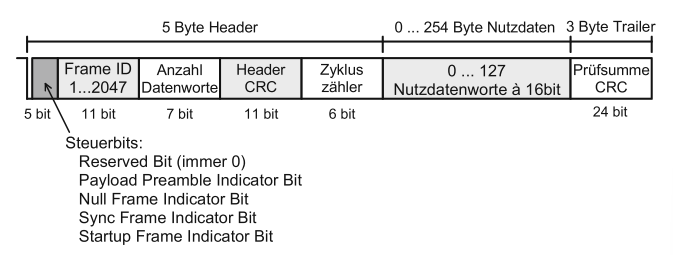
\includegraphics[width=\textwidth]{Zimmermann_FlexrayBotschaft}
\label{fig:FlexRayBotschaft}
\caption{Aufbau einer FlexRay-Botschaft}
\quelle{\cite[101]{Zimmermann.2014}}
\end{figure}


\subsection{Media Oriented System Transport}
Das \ac{MOST} Protokoll wird vor allem in Infotainment-Systemen von Autos eingesetzt. Anstelle von Kabeln werden hier Lichtwellenleiter verwendet. Somit ist das Signal unempfänglich gegenüber elektromagnetischer Einstrahlung. Es wird unterschieden zwischen \acs{MOST}25, \acs{MOST}50 und \acs{MOST}150, welche sich in Paketgröße und Bandbreite unterscheiden. Ein \acs{MOST}-Netzwerk ist meist als Ringtopologie aufgebaut (vergleiche Abbildung \ref{fig:MOST-NetworkMasterSlave}). Auch im \acs{MOST}-Protokoll gibt es Master- und Slave-Knoten. Der Master-Knoten ist häufig ein Gateway zu einem \acs{CAN}-Bus.\\

\begin{figure}[H]
\centering
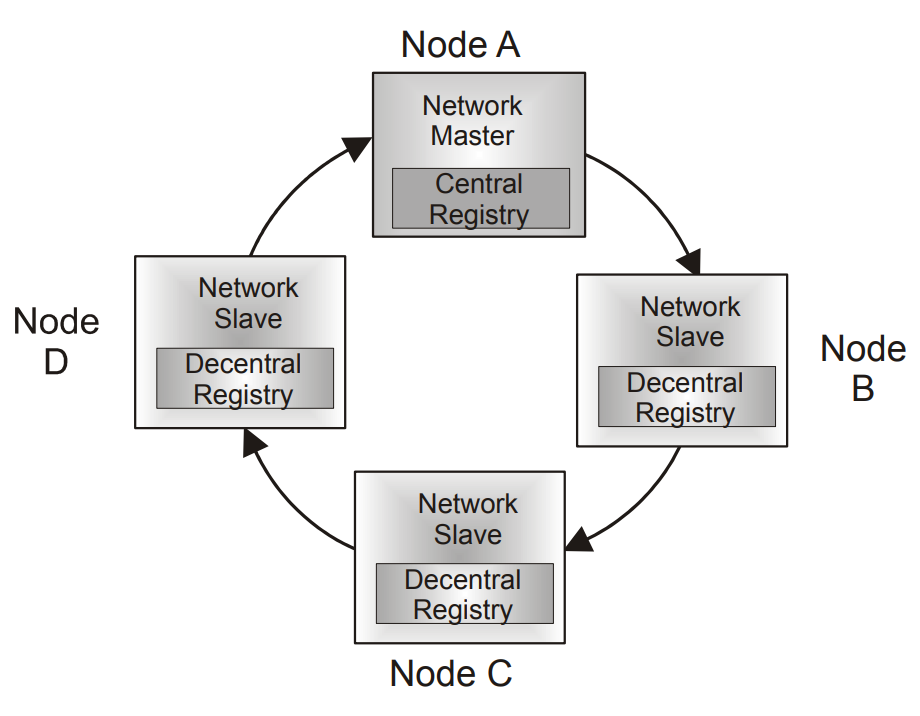
\includegraphics[width=0.7\textwidth]{Grzemba_MOST_NetworkMasterSlave}
\label{fig:MOST-NetworkMasterSlave}
\caption{Ringtopologie eines \acs{MOST}-Bus}
\quelle{\cite[40]{Grzemba.2007}}
\end{figure}

\subsubsection{Paketaufbau}
Der Aufbau eines \acs{MOST}25-Pakets ist in Abbildung \ref{fig:MOST-frame} dargestellt. Es folgt eine kurze Erklärung der Einzelnen Bestandteile.
\subparagraph{Anfangsfeld (Preamble)} Das Anfangsfeld wird vom TimingMaster generiert und dient der Synchronisation der Slaves.
\subparagraph{Abgrenzungsfeld (Boundary Descriptor)}Das Abgrenzungsfeld definiert die in Vier-Byte-Schritten verschiebbare Grenze zwischen Stream- und Paketdaten.
\subparagraph{Datenfeld (stream data, packet data)}Das Datenfeld besteht aus 60 Bytes die nach Bedarf zwischen Streamdaten und Paketdaten aufgeteilt werden können.
\subparagraph{Kontrollbytes (Frame Control)}Die Kontrollbytes am Ende dienen der Kontrolle des Frames.
\subparagraph{Paritätsfeld (Parity Bit)}Das Paritätsfeld ermöglicht das Erkennen von Bit-Fehlern im Frame.
\\

\begin{figure}[H]
\centering
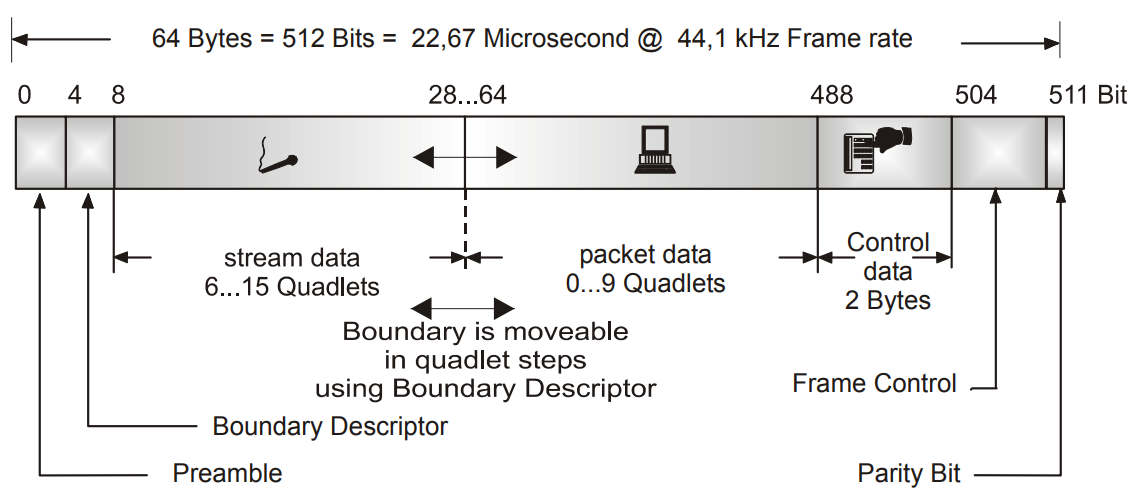
\includegraphics[width=\textwidth]{Grzemba_MOST_frame}
\label{fig:MOST-frame}
\caption{Aufbau eines \acs{MOST}25-Pakets}
\quelle{\cite[88]{Grzemba.2007}}
\end{figure}


\subsection{Automotive Ethernet}
Die Vielzahl inkompatibler und nur in der Automobilindustrie verwendeter Lösungen resultierte in hohen Kosten und kontinuierlichem Weiterentwicklungsaufwand. Zudem steigt der Bandbreitenbedarf. Daher wird das bereits im Bürobereich etablierte Konzept Ethernet/IP relevanter für den Automobilbereich. \cite[138]{Zimmermann.2014}\\
Die in diesem Standard verwendeten Protokolle \ac{IP}, \ac{TCP} und \ac{UDP} werden außerdem schon von den meisten computerähnlichen Geräten unterstützt. Das ermöglicht eine transparente Kommunikation und vereinfacht die Integration von Consumergeräten erheblich \cite{Zimmermann.2014}. Ethernet war ursprünglich ein Linienbussystem, wird heutzutage aber meistens als Sterntopologie mit Switches an Kopplungspunkten umgesetzt. \\
In Abbildung \ref{fig:EthernetPaket} ist der Aufbau eines Ethernet-Pakets dargestellt. 
Die Präambel und der Start Frame Delimiter spielen eine Rolle bei der Taktsynchronisation bei manchen Physical Layern. Die Ziel- und Quell-MAC-Adresse dienen der Geräteadressierung. Das VLAN-Tag erlaubt die Bildung von Unternetzen. Das Typfeld kennzeichnet den Typ des Inhalts des darauf folgenden Datenfelds. Das Datenfeld enthält den eigentlichen Nachrichteninhalt. Am Ende jedes Pakets befindet sich noch die Frame Check Sequence zur Detektion von Übertragungsfehlern. Beim Eintritt eines Übertragungsfehlers wird die Botschaft automatisch vom Empfänger verworfen. \cite[140]{Zimmermann.2014}\\

\begin{figure}[H]
\centering
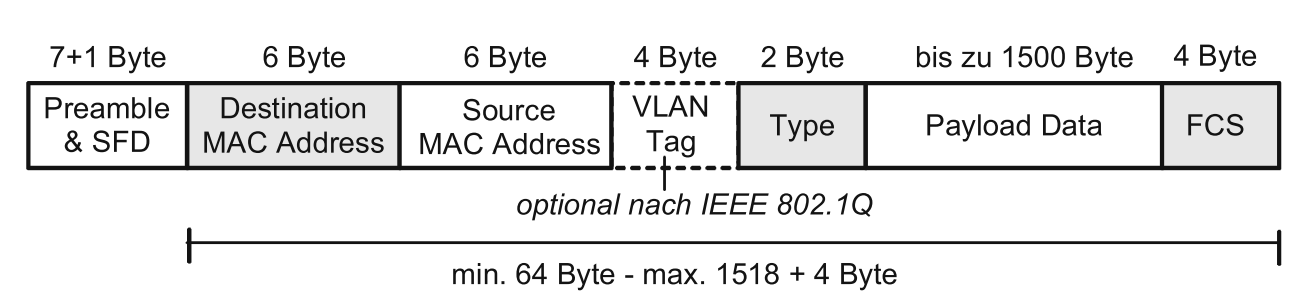
\includegraphics[width=\textwidth]{Zimmermann_EthernetPaket}
\label{fig:EthernetPaket}
\caption{Aufbau eines Ethernet-Pakets}
\quelle{\cite[140]{Zimmermann.2014}}
\end{figure}



\section{Schnittstellen}\label{Schnittstellen}
Moderne Autos verfügen über eine Vielzahl von Schnittstellen, um eine Verbindung mit dem Fahrzeug herzustellen, sei es, um ein Multimediagerät zu verbinden oder zu Diagnosezwecken. Diese Schnittstellen können aber auch eventuell einem potentiellen Angreifer den Zugriff auf das Fahrzeugnetzwerk ermöglichen. Diese möglichen Angriffsvektoren können nach Checkoway et al \cite[1]{Checkoway.2011} in drei Kategorien eingeteilt werden. Diese drei Kategorien sind \glqq indirect physical access\grqq , \glqq short-range physical access\grqq{} und \glqq long-range physical access\grqq . Es folgt eine Beschreibung der Kategorien mit einer Übersicht der typischsten Schnittstellen eines modernen Autos.

\subsection{Indirect Physical Access}
Zu dieser Kategorie zählen sämtliche physische Schnittstellen, die direkt oder indirekt auf die internen Netzwerke des Autos zugreifen. Bei diesen Schnittstellen müsste ein Angreifer, um darauf zuzugreifen, mindestens einmalig physischen Zugang zum Fahrzeug haben oder über einen Vermittler arbeiten. 


\subsubsection{OBD-II Port} \label{OBD-II}
Der \ac{OBD}-II Port ist eine für Fachleute gedachte Schnittstelle auf den \acs{CAN}-Bus zu Diagnosezwecken.	Er befindet sich meist im Fußraum auf der Fahrerseite. Der Port umfasst 16 Pins, obwohl durch den Standard nur die Belegung von neun Pins vorgeschrieben ist. Die zusätzlichen Pins werden je nach Anbieter teilweise für den Zugriff auf zusätzliche Bussysteme verwendet. \cite[2]{Klinedinst.2016} \\
Üblicherweise wird an diesen Port ein Diagnosegerät des Herstellers oder einer Werkstatt angeschlossen. Das Diagnosegerät wird entweder von meist Windows-basierten Personal Computern programmiert oder fungieren als Mittler, um direkt mittels Laptop auf Port zuzugreifen \cite[3]{Checkoway.2011}. In beiden Fällen hat ein Windows-basierter PC direkt oder indirekt Zugriff auf das Netzwerk des Fahrzeugs. Der Hauptzweck dieses Gerätes ist es, Daten aus den \acsp{ECU} des Fahrzeugs zu sammeln. Das erfolgt über das Senden von diagnostischen \acs{CAN}-Paketen. Die betroffenen \acsp{ECU} senden anschließend die angefragten Daten. Diese Daten können dann beispielsweise zur Behandlung von Problemen verwendet werden.\\
Verbrauchermarktanbieter konnten allerdings die Kommunikationsarchitektur durch Reverse-Engineering verstehen und für andere Zwecke nutzen, zum Beispiel Pay-By-Mile-Versicherungen, Fahrzeuggebrauchstracking und kommerzielles Flottenmanagement \cite[3]{Klinedinst.2016}. \\

\subsubsection{Ladeanschluss eines Elektro-Autos}
Elektronische Fahrzeuge tanken nicht an Tankstellen wie ihre kraftstoffbetriebenen Pendants, sondern können an einer Steckdose oder speziellen, teilweise öffentlichen Ladestationen aufgeladen werden. Beim Ladevorgang an Ladestationen werden allerdings nicht nur elektrischer Strom sondern auch Daten ausgetauscht \cite[3]{Checkoway.2011}. Beispiele dafür können die Steuerung des Ladevorgangs, Authentifizierung und Autorisierung und Informationen über Ladezeit, Ladeleistung, Energieverbrauch und Batteriezustand sein. Dieser Datenaustausch ermöglicht einen effizienten und sicheren Ladevorgang, eine Abrechnung des bereitgestellten Stroms und eine Überwachung der Ladeinfrastruktur. Zudem können eine unautorisierte Nutzung der Ladestation oder eine Überlastung des Stromnetzes verhindert werden. 

\subsubsection{Entertainment}
Eine Vielzahl der physischen Schnittstellen eines Autos ist außerdem der Unterhaltung des Benutzers gewidmet. Beispielsweise bieten die meisten Autos mindestens einen USB- und einen Aux-Anschluss, damit Musik von externen Geräten abgespielt werden kann. Außerdem sind viele Autos mit einem CD-Laufwerk ausgestattet. Meist werden mehrere Audioformate unterstützt. Häufig sind die Entertainment-Systeme mit einem \acs{CAN}-Bus verbunden \cite[4]{Checkoway.2011}, um beispielsweise ganzheitliche Firmwareupdates zu ermöglichen. Außerdem kann das Infotainment-System Informationen von anderen Fahrzeugsystemen abrufen, um dem Fahrer relevante Daten anzuzeigen. Dazu gehören Informationen wie Fahrzeuggeschwindigkeit, Motordrehzahl oder Kraftstoffverbrauch, die dann auf dem Display angezeigt werden können.

\subsection{Short-Range Wireless Access}
Diese Kategorie umfasst Schnittstellen, deren Nutzung zwar drahtlos erfolgt, aber dennoch eine geringe physische Distanz zum Fahrzeug erfordert. Ein potenzieller Angreifer müsste sich für die Nutzung dieser Schnittstellen entweder in der Nähe befinden oder einen Transmitter in der Umgebung platzieren.


\subsubsection{Bluetooth}
Um Features wie eine Freisprecheinrichtung oder das Hören eigener Musik vom Smartphone zu realisieren, bieten die Infotainment-Systeme der meisten modernen Autos eine Bluetooth-Schnittstelle. Bluetooth ermöglicht die drahtlose Kommunikation zwischen dem Fahrzeug und externen Geräten wie Smartphones. Durch die Verbindung des Infotainment-Systems mit dem Controller Area Network des Fahrzeugs kann es mit anderen elektronischen Steuergeräten (\acsp{ECU}) kommunizieren. Diese Integration ermöglicht eine nahtlose Interaktion zwischen dem Infotainment-System und anderen Fahrzeugsystemen.
Die Bluetooth-Verbindung eröffnet Möglichkeiten für die Nutzung von verschiedenen Funktionen und Diensten. Eine der häufigsten Anwendungen ist die Freisprecheinrichtung, die es dem Fahrer ermöglicht, Anrufe über das Infotainment-System zu tätigen und entgegenzunehmen, ohne das Telefon in die Hand nehmen zu müssen. Das Infotainment-System wird über Bluetooth mit dem Telefon gekoppelt und kann auf die Telefonkontakte zugreifen, Anrufe initiieren und Anrufinformationen auf dem Display anzeigen.
Darüber hinaus ermöglicht die Bluetooth-Schnittstelle auch die drahtlose Übertragung von Audiodateien vom Smartphone zum Infotainment-System. Fahrer und Insassen können ihre eigenen Musikbibliotheken, Streaming-Dienste oder Podcasts über das Fahrzeuglautsprechersystem abspielen. Das Infotainment-System fungiert als Empfänger für das Audiosignal, das vom Smartphone gesendet wird.

\subsubsection{Remote Keyless Entry}
\ac{RKE} Systeme, auch als Funkfernbedienung oder Keyless-Entry-Systeme bekannt, sind Technologien, die es Fahrzeugbesitzern ermöglichen, ihr Fahrzeug aus der Ferne zu verriegeln und zu entriegeln, ohne einen physischen Schlüssel verwenden zu müssen. Diese Systeme bieten eine bequeme und sichere Möglichkeit, auf das Fahrzeug zuzugreifen.
Ein typisches RKE-System besteht aus zwei Hauptkomponenten: einem Funksender (Fernbedienung) und einem Empfänger, der im Fahrzeug eingebaut ist. Die Fernbedienung ist normalerweise eine kleine tragbare Vorrichtung, die über eine oder mehrere Tasten verfügt. Durch Betätigen der Tasten sendet die Fernbedienung ein verschlüsseltes Funksignal mit einer bestimmten Reichweite an den Empfänger im Fahrzeug.
Der Empfänger im Fahrzeug erkennt das Signal der Fernbedienung und interpretiert es. Wenn das empfangene Signal korrekt und authentifiziert ist, führt das RKE-System die gewünschte Aktion aus. Das kann das Entriegeln oder Verriegeln der Türen, das Aktivieren oder Deaktivieren der Diebstahlalarmanlage oder das Öffnen der Kofferraumklappe sein. In einigen Fahrzeugen können auch weitere Funktionen über die Fernbedienung gesteuert werden, wie das Starten des Motors oder das Ein- und Ausschalten der Fahrzeugbeleuchtung.\\
Des Weiteren sind viele moderne Automobile mit sogenannten Passive Keyless Entry and Start Systemen ausgestattet. Diese basieren auf einem bidirektionalen Challenge-Response-Schema. Das Auto sendet eine Challenge, woraufhin der Autoschlüssel mit einer kryptographischen Antwort (Response) reagiert. Bei einer gültigen Antwort werden die Türen entriegelt, das Alarmsystem deaktiviert und das Starten des Motors ermöglicht. Eine Benutzerinteraktion ist nicht notwendig, der Schlüssel muss sich lediglich in einem Umkreis von in der Regel etwa einem Meter zum Fahrzeug befinden. \cite[930]{Garcia.2016} \\
RKE-Systeme nutzen verschiedene drahtlose Kommunikationstechnologien wie Radiofrequenz (RF) oder Infrarot (IR), um die Signale zwischen der Fernbedienung und dem Fahrzeug zu übertragen \cite[4]{Checkoway.2011}. RF-basierte Systeme sind am weitesten verbreitet, da sie eine größere Reichweite bieten und nicht auf Sichtverbindung angewiesen sind.

\subsubsection{Reifendruck-Kontrollsystem}
Ein weiteres drahtloses Netzwerk in Fahrzeugen stellt das \ac{RDKS} oder auf englisch Tire Pressure Monitoring System (TPMS) dar. Die Integration eines solchen Systems ist in vielen Ländern gesetzlich vorgeschrieben. Neben der Vermeidung von Reifenpannen verspricht die Warnung vor falschem Reifendruck eine Steigerung der Verkehrssicherheit und Kraftstoffeffizienz, da der richtige Reifendruck die Traktion, den Bremsweg und den Rollwiderstand verbessert. Das Reifendrucküberwachungssystem misst kontinuierlich den Luftdruck in allen Reifen von Personenkraftwagen, Lastwagen und Mehrzweckfahrzeugen und warnt den Fahrer, wenn ein Reifen signifikant zu wenig aufgepumpt ist. Es gibt sowohl direkte als auch indirekte Messverfahren. Bei einem direkten Messsystem werden batteriebetriebene Drucksensoren in jedem Reifen verwendet, um den Reifendruck zu messen, und die Daten werden über einen Funkfrequenz (RF)-Sender übertragen, da eine Verkabelung von einem rotierenden Reifen zur elektronischen Steuereinheit des Fahrzeugs schwierig umzusetzen ist. Die empfangende Reifendrucksteuereinheit analysiert die Daten und kann über das \ac{CAN} Ergebnisse oder Befehle an den zentralen Bordcomputer senden, um beispielsweise eine Warnmeldung auf dem Fahrzeugdashboard auszulösen. Indirekte Messsysteme leiten den Druckunterschied zwischen den Reifen aus den Unterschieden in der Rotationsgeschwindigkeit ab, die mithilfe der \ac{ABS}-Sensoren gemessen werden können. Ein Reifen mit niedrigerem Druck muss schneller rotieren, um die gleiche Strecke wie ein Reifen mit höherem Druck zurückzulegen. Die Nachteile dieses Verfahrens sind jedoch eine geringere Genauigkeit, die Kalibrierung durch den Fahrer und die Unfähigkeit, den gleichzeitigen Druckverlust in allen Reifen zu erkennen. Daher werden primär direkte Reifenkontrollsysteme verwendet. \cite[1]{Rouf.2010}

\subsubsection{Wireless LAN}
Viele Hersteller statten ihre modernen Autos heutzutage mit einer \ac{WLAN}-Schnittstelle aus \cite[4]{Checkoway.2011}. Die Technologie wird für verschiedene Anwendungsfälle eingesetzt. Viele moderne Autos sind mit Infotainment-Systemen ausgestattet, die WLAN verwenden, um eine drahtlose Verbindung zum Internet herzustellen. Dadurch können Insassen auf Streaming-Dienste, Musik, Online-Radio, und andere Online-Inhalte zugreifen. \acs{WLAN} ermöglicht auch Over-the-Air-Updates für das Infotainment-System, um Softwareaktualisierungen und neue Funktionen bereitzustellen. Auch für den Rest des Fahrzeugs lassen sich je nach Modell teilweise Softwareupdates über \acs{WLAN} herunterladen. Zum Beispiel die Autos von Tesla bieten dieses Feature. Darüber hinaus ermöglicht \acs{WLAN} den Passagieren im Auto in manchen Fahrzeugen die drahtlose Verbindung ihrer mobilen Geräte wie Smartphones, Tablets und Laptops mit dem Internet.
Schließlich werden \acs{WLAN}-basierte Standards ebenfalls in der Fahrzeug-zu-Fahrzeug-Kommunikation eingesetzt. Diese Art der Kommunikation wird auch Dedicated Short-Range Communications (DSRC) genannt \cite[4]{Checkoway.2011}. Durch den Datenaustausch zwischen Fahrzeugen sollen beispielsweise Kollisionen frühzeitig erkannt und verhindert werden. \\
Um die genannten Features umsetzen zu können, ist größtenteils eine Verbindung der \acs{ECU} mit der \acs{WLAN}-Schnittstelle zum Controller Area Network notwendig. Somit kann in vielen Fahrzeugen auch über \acs{WLAN} theoretisch indirekt auf den \acs{CAN}-Bus zugegriffen werden.



\subsection{Long-Range Wireless Access}
Zu dieser letzten Kategorie zählen alle Zugriffskanäle, die aus großer Entfernung, nämlich mehr als einem Kilometer, zugegriffen werden kann. Immer mehr Autos bieten auch derartige Schnittstellen. Diese lassen sich in zwei Kategorien einteilen: Broadcast Kanäle und Adressierbare Kanäle. \cite[4]{Checkoway.2011}

\subsubsection{Broadcast Kanäle}
Broadcast Kanäle sind Kanäle, die nicht speziell auf ein bestimmtes Fahrzeug ausgerichtet sind, sondern von Empfängern nach Bedarf empfangen werden können. 
Das moderne Automobil umfasst eine Vielzahl von Empfängern für weit reichende Broadcast-Signale: \ac{GPS}, Satellitenradio, Digitalradio und das Radio Data System (RDS) und der Traffic Message Channel (TMC), die als digitale Unterträger auf vorhandenen FM-Bändern übertragen werden. Die Reichweite solcher Signale hängt von der Sendeleistung, Modulation, Gelände und Störungen ab. Im Allgemeinen werden diese Kanäle in das Mediasystem eines Autos (Radio, CD-Player, Satellitenempfänger) implementiert, das, wie bereits erwähnt, häufig über interne Automobilnetzwerke Zugriff auf andere wichtige \acsp{ECU} ermöglicht. \cite[4\psq]{Checkoway.2011}

\subsubsection{Adressierbare Kanäle}
Über adressierbare Kanäle lassen sich individuelle Fahrzeuge direkt ansteuern. Die Verbindung erfolgt in der Regel über das Mobilfunknetz.\\
Durch diese Kanäle können viele Funktionen bereitgestellt werden. Dazu gehören die Unterstützung von Sicherheit (Unfallberichterstattung), Diagnose (frühzeitige Warnung bei mechanischen Problemen), Diebstahlschutz (Fernverfolgung und Deaktivierung) und Komfort (Zugriff auf Daten wie Fahrtrichtungen oder Wetterinformationen). \cite[5]{Checkoway.2011} \\
Da diese Kanäle meist eine hohe Bandbreite bieten, über große Distanzen und in beide Richtungen funktionieren und das direkte Ansteuern von individuellen Fahrzeugen ermöglichen, sind diese Schnittstellen für potenzielle Angreifer besonders interessant \cite[5]{Checkoway.2011}.

%evt Automatisiertes/autonomes Fahren

%evt Architektur


\section{Cyber Security}
Als nächstes werden die Grundlagen der Cyber Security und IT Sicherheit erläutert, die im Bereich der Automotive Security relevant sind. Die IT Security befasst sich eher mit der Sicherheit von elektronisch gespeicherten Daten während die Cyber Security diese Sicherheit auf ganze Systeme, Netzwerke und Kommunikation ausweitet.
Die Begriffe Cyber- und IT Security sind jedoch eng miteinander verwandt und werden häufig als Synonym verwendet.

\subsection{Security und Safety}
Der deutsche Begriff \glqq Sicherheit\grqq{} ist mehrdeutig, was ihn für eine genaue, technische Definition ungeeignet macht. In der IT-Sicherheit wird zwischen den beiden englischen Begriffen \glqq Safety\grqq{} und \glqq Security\grqq{} unterschieden.
\subparagraph{Safety}
\glqq Der Begriff Safety bezeichnet die funktionale Sicherheit, bzw. die Betriebssicherheit eines Systems. Ein System darf seine Umgebung etwa durch undefiniertes, unzulässiges Verhalten oder Zustände nicht gefährden. Safety schützt somit Mensch und Umwelt vor negativen Einflüssen des Systems, etwa durch Fehlverhalten und Ausfälle.\grqq{} \cite[2]{Wurm.2022}
\subparagraph{Security}
\glqq Der Begriff Security bezeichnet die Informations- und Datensicherheit bzw. die Angriffssicherheit eines Systems. Security umfasst alle Eigenschaften und Maßnahmen, die das System vor absichtlichen und unabsichtlichen Bedrohungen
von außen schützen. Security schützt somit das System vor negativen Einflüssen von Mensch und Umwelt, wie etwa Bedrohungen und Angriffe. Während sich die sog. klassische IT-Security auf die Absicherung der informationstechnischen Systeme eines Unternehmens wie etwa Computer, Server, Netzwerke und Internetanbindungen konzentriert, zielt die Cybersecurity im Kontext des Automotive Bereichs auf die Absicherung deren Produkte ab.\grqq{} \cite[2\psq]{Wurm.2022}\\

Safety bezieht sich somit mehr auf die Sicherheit des Nutzers während sich die Security eines Systems mehr auf die Sicherheit von Daten, Informationen und des Systems an sich fokussiert. Im Automotive-Kontext ist Security in vielen Fällen eine Voraussetzung für die Safety von Fahrzeugen, da durch Security-Maßnahmen verhindert werden soll, dass das Fahrzeug in einen Safety-kritischen Zustand gebracht wird. In anderen Fällen stehen sich Safety- und Security-Ziele aber auch teilweise gegenseitig im Weg. Zum Beispiel kann durch erhöhte Security-Maßnahmen die Latenz der Fahrzeugsysteme ansteigen, was sich wiederum negativ auf die Safety auswirkt. Daher kann es eine Herausforderung sein, beide Disziplinen gemeinsam ausreichend zu behandeln.

%evt Authentisierung, Authentifizierung, Autorisierung
\subsection{Sicherheitsziele}\label{Sicherheitsziele}
Die Sicherheitsziele beschreiben Eigenschaften von Informationen und anderen schützenswerten Ressourcen, die gewünscht sind, um Sicherheit zu gewährleisten. Security-Maßnahmen sollten darauf ausgelegt sein, diese Ziele zu erreichen. Faktoren, die das Erreichen der Sicherheitsziele gefährden, können als Bedrohung identifiziert werden. Die klassischen Sicherheitsziele in der IT Security sind Vertraulichkeit, Integrität und Verfügbarkeit (siehe Abbildung \ref{fig:Sicherheitsziele}). Diese Ziele werden manchmal auch als CIA-Ziele bezeichnet. CIA entspricht hierbei der Abkürzung der englischen Begriffe Confidentiality, Integrity und Availability. Im Automotive Bereich werden allerdings oft zusätzlich die Ziele Authentizität, Zurechenbarkeit und Schutz der Privatsphäre genannt \cite[6]{Wurm.2022}. \\

\begin{figure}[H]
\centering
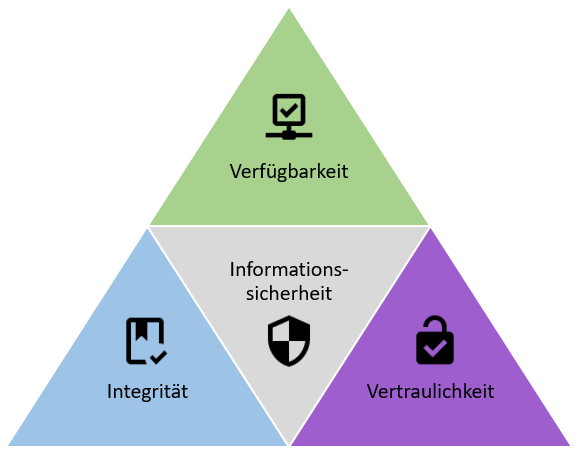
\includegraphics[width=0.5\textwidth]{Sicherheitsziele}
\label{fig:Sicherheitsziele}
\caption{Die drei klassischen Sicherheitsziele der IT Security}
\quelle{\cite{Pukies.2020}}
\end{figure}

\subsubsection{Vertraulichkeit}
\glqq  Vertraulichkeit beschreibt die Eigenschaft, dass ausschließlich berechtigte Personen bzw. Entitäten auf die zu schützenden Informationen zugreifen können.
\grqq{} \cite[7]{Wurm.2022}\\
Dieses Sicherheitsziel kann durch unterschiedliche Maßnahmen erreicht werden, die sich teilweise gegenseitig ergänzen. Dazu gehören zum Beispiel Zugriffskontrollen, Verschlüsselung und Verstecken der Informationen.\\
Es kann verschiedene Gründe geben, warum manche Informationen vertraulich bleiben sollen. So kann durch das Bekanntwerden gewisser Informationen zum Beispiel ein wirtschaftlicher Schaden entstehen. Das kann der Fall sein bei geistigem Eigentum oder auch Firmengeheimnissen. Außerdem schützenswert sind personenbezogene Daten.

\subsubsection{Integrität}
\glqq Integrität beschreibt den Schutz von Informationen vor unbeabsichtigten oder böswilligen Veränderungen.
\grqq{} \cite[7]{Wurm.2022} \\
Das Wort Veränderungen schließt hierbei auch das Entfernen oder Hinzufügen von Daten ein, somit gelten diese Aktionen ebenfalls als Verletzung der Integrität.
Um die Integrität schützenswerter Informationen zu gewährleisten, werden technische Maßnahmen wie kryptographische Checksummen eingesetzt. Dadurch kann zwar ein Verlust der Integrität nicht verhindert werden, jedoch kann er zweifelsfrei und nicht kompromittierbar erkannt werden. Der Schutz der Integrität spielt eine entscheidende Rolle für die korrekte Funktionsweise der gesamten ECU-Software und insbesondere für sicherheitsrelevante Informationen.

\subsubsection{Verfügbarkeit}
\glqq Verfügbarkeit (engl. availability) definiert die Anforderung an das System, seine Dienste und Funktionen innerhalb einer gewissen Zeitspanne (Echtzeitfähigkeit) nach Aufforderung zur Verfügung stellen zu können.
\grqq{} \cite[7]{Wurm.2022} \\
Um einen reibungslosen und sofortigen, teilweise sogar Echtzeit-, Betrieb zu gewährleisten, müssen Hardware-, Software- und Kommunikationsressourcen verfügbar sein. Häufig ist das Ziel eines Angreifers, den Dienst einzuschränken oder vollständig zu verweigern. Eine gängige technische Lösung zur Aufrechterhaltung der Verfügbarkeit ist zum Beispiel die Implementierung redundanter Pfade. Wenn ein Primärsystem ausfällt, kann ein redundantes (Teil-)System die Aufgabe übernehmen und so die Verfügbarkeit sicherstellen.

\subsubsection{Authentizität}
\glqq  Authentizität bedingt, dass die Echtheit einer Information bzw. eines Absenders sichergestellt ist. Die Authentizität einer Information ist gegeben, falls dessen Urheber eindeutig identifizierbar und dessen Urheberschaft kryptographisch sicher überprüfbar ist.
\grqq{} \cite[7]{Wurm.2022} \\
Die Authentizität von Informationen ist eng mit der Integrität von Informationen verwandt. Technisch kann Authentizität durch digitale Signatur oder Zertifikate umgesetzt werden.

\subsubsection{Zurechenbarkeit}
\glqq Zurechenbarkeit bzw. Verbindlichkeit (engl. accountability) ist eine Eigenschaft, die dafür garantiert, dass die entsprechende Person oder Entität die Urheberschaft einer bestimmten Information bzw. eine bestimmte Aktion nicht von sich weisen kann.
\grqq{} \cite[8]{Wurm.2022} \\
Der Begriff Nichtabstreitbarkeit wird oft ähnlich verwendet, spielt jedoch insbesondere in rechtlichen Angelegenheiten wie Haftung und Gewährleistung eine Rolle. Es wurde festgestellt, dass die Abstreitbarkeit eine potenzielle Schwachstelle darstellt. Wenn zum Beispiel der Empfang oder das Senden bestimmter kritischer Nachrichten, wie Warnungen vor Stauenden oder Geschwindigkeitsbegrenzungen, bestritten werden kann, ist eine rechtssichere Zuordnung nicht möglich und eine mögliche Strafverfolgung wird erschwert. Ohne das Schutzziel der Nichtabstreitbarkeit könnte jeder Teilnehmer bestreiten, eine bestimmte Nachricht gesendet oder empfangen zu haben. Die technische Umsetzung kann durch manipulationssichere Log-Speicher erfolgen, die den Empfang bestimmter Nachrichten protokollieren und nachweisen können. Die Nichtabstreitbarkeit der Urheberschaft einer gesendeten Nachricht wird durch das digitale Signaturverfahren in Verbindung mit einer vertrauenswürdigen Public-Key-Infrastruktur gewährleistet. \cite[8]{Wurm.2022}

\subsubsection{Schutz der Privatsphäre}
Moderne Fahrzeuge und Hersteller erheben, verarbeiten und speichern personenbezogene Daten. Beispielsweise wird die Position des Autos im Rahmen der \ac{V2X}-Kommunikation zyklisch veröffentlicht. Hierbei ist es zum einen im Interesse der betroffenen Person, des Fahrers, dass sich diese Daten sich nicht zu den betroffenen Personen zuordnen lassen. Außerdem ist es aber auch durch die Datenschutzgrundverordnung, die im Jahr 2018 in Kraft trat, gesetzlich vorgeschrieben. Technisch lässt sich der Schutz der Privatsphäre zum Beispiel mit einer Tarnidentität umsetzen.


\subsection{Risikomanagement}
Der systematische Umgang mit Gefahren und Risiken ist ein wichtiger Bestandteil des Cybersecurity-Engineering-Prozesses. Im Kontext von Cybersecurity-Angriffen beziehen sich Bedrohungen, Schwachstellen und Risiken auf verschiedene Aspekte. Die schützenswerten Güter eines Systems, auch genannt Assets, können sowohl materieller als auch immaterieller Natur sein, wie zum Beispiel sensible Informationen, Fahrzeugfunktionen, Softwarekomponenten, Hardwarekomponenten, Infrastrukturkomponenten und Kommunikationsverbindungen. Risikobewertungsmodelle definieren die Sicherheitseigenschaften der Assets, wie Vertraulichkeit, Integrität und Verfügbarkeit (vergleiche Kapitel \ref{Sicherheitsziele}), und legen ihren Schutzbedarf fest. \cite[5]{Wurm.2022}\\
Bedrohungen können absichtliche oder unabsichtliche Ereignisse sein, die die Schutzziele der Assets beeinträchtigen können, sei es durch bösartige Aktivitäten von Angreifern oder unvorhersehbare Ereignisse wie Ausfälle oder physische Beschädigungen. \\
Angreifer nutzen vorhandene Schwachstellen aus, um Angriffe durchzuführen und die Assets eines Systems zu bedrohen. Passive Angriffe zielen hierbei auf die Informationsbeschaffung ab, während aktive Angriffe darauf abzielen, die Integrität, Authentizität und Verfügbarkeit des Systems zu beeinträchtigen. \\
Risiken werden im Rahmen einer Risikoanalyse bewertet und sind definiert durch Eintrittswahrscheinlichkeit und potenzielles Schadensausmaß. Schwachstellen erhöhen das Risiko, während Gegenmaßnahmen und Schutzkonzepte das Risiko reduzieren. Gegenmaßnahmen, auch als Sicherheitskontrollen bezeichnet, sollen potenzielle Bedrohungen verhindern und die Wahrscheinlichkeit von Angriffen auf ein akzeptables Niveau reduzieren. Angreifer können aus verschiedenen Personengruppen stammen, von Hobby-Hackern bis hin zu staatlichen Organisationen wie Geheimdiensten. Es ist jedoch auch möglich, dass Angriffe von aktuellen Fahrzeugbesitzern selbst durchgeführt werden, beispielsweise durch das Manipulieren des Kilometerstandes zur Erhöhung des Wiederverkaufswerts eines Fahrzeugs. \cite[5\psq]{Wurm.2022}

\subsubsection{Risikomatrix}
Ein sehr verbreitetes Werkzeug der Risikoanalyse ist die Risikomatrix (siehe Abbildung \ref{fig:Risikomatrix}). Sie dient der Einschätzung und Berechnung von Risiken. Mithilfe einer Risikomatrix kann die Bedeutung und das Ausmaß eines Risikos einfach bestimmt und anschaulich visualisiert werden. In der Regel hat eine Risikomatrix die zwei Dimensionen Eintrittswahrscheinlichkeit und Schadensausmaß. Diese verfügen meist über eine vorher zu definierende, künstliche, ordinale Skalierung. Die Risiken werden dann auf einer Skala von niedrig bis hoch in Bezug auf ihre Wahrscheinlichkeit und Auswirkung eingestuft. Die Wahrscheinlichkeit kann beispielsweise in Kategorien wie selten, gelegentlich, häufig oder sehr häufig unterteilt werden, während die Auswirkung auf Kategorien wie gering, moderat, hoch oder katastrophal abgestuft werden kann. Die einzelnen Felder der Matrix sind meist in verschiedenen Farben eingefärbt. Die genaue Farbverteilung der Felder innerhalb der Matrix ist individuell und kann sich je nach Anwendungsfall unterscheiden. In der Regel sind geringe Risiken grün, mittlere Risiken gelb und große Risiken rot eingefärbt. Wo genau die Grenze gezogen wird ist jedoch dem Ersteller überlassen.
Die Risikobewertung erfolgt durch das Zuweisen eines Wertes oder einer Farbe zu jedem Risiko, abhängig von seiner Position in der Risikomatrix. Für die Berechnung eines Wertes wird meist der Wert der Eintrittswahrscheinlichkeit mit dem Wert des Schadensausmaßes multipliziert. Abhängig von der Klassifikation eines Risikos kann anschließend entschieden werden, wie es zu behandeln ist.
\\

\begin{figure}[H]
\centering
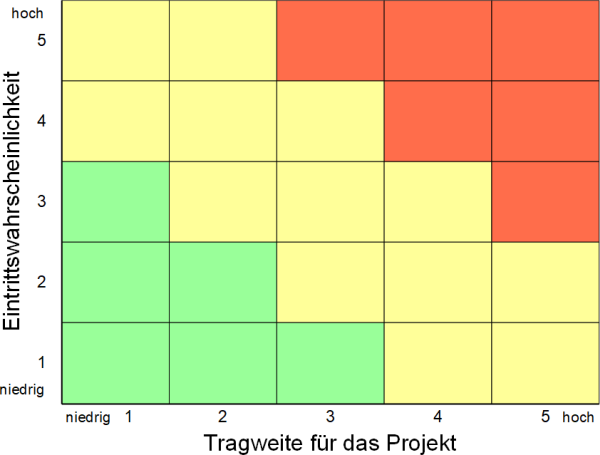
\includegraphics[width=0.7\textwidth]{Risikomatrix}
\label{fig:Risikomatrix}
\caption{Beispiel für eine Risikomatrix}
\quelle{\cite{Peterjohann.2014}}
\end{figure}

%\subsection{ISMS}
%\cite[62]{Wurm.2022} (Kapitel 3)

\subsection{Kryptographie}
\glqq Der Begriff Kryptographie stammt vom griechischen kryptos (verborgen) und graphein (schreiben) ab und bezeichnet die Wissenschaft der Geheimschriften oder der Verschlüsselung von Informationen.
\grqq{} \cite[9]{Wurm.2022}\\
Die Kryptographie beschäftigt sich also hauptsächlich damit, Informationen in anderer Form darzustellen. Dies kann Zwecken der Geheimhaltung, Datenübertragung oder Komprimierung dienen. Außerdem können kryptographische Verfahren wie zum Beispiel RSA auch zur Authentifizierung durch Signaturen eingesetzt werden.\\
Kryptographie im Zusammenhang mit der Sicherheit von Kraftfahrzeugen bezieht sich auf den Einsatz von Ver- und Entschlüsselungstechniken zur Gewährleistung der Vertraulichkeit, Integrität und Authentizität von Daten und Kommunikationssystemen in Fahrzeugen. Durch den Einsatz kryptografischer Techniken werden Informationen vor unbefugtem Zugriff und Manipulationen geschützt, um die Sicherheit und Privatsphäre der Fahrzeuginsassen zu gewährleisten. \\
Hierbei gilt wie in der allgemeinen IT Security das Auguste Kerkhoff Prinzip. Dieses besagt, dass in einem guten Kryptographiesystem lediglich der Schlüssel geheim gehalten werden muss. Das System muss auch dann Sicherheit bieten, wenn seine genaue Funktionsweise bekannt ist. Das Prinzip \glqq Security by Obscurity\grqq , also Sicherheit durch Verschleierung der Funktionsweise des Kryptographiesystems, sollte nicht zum Einsatz kommen. Daher beruhen viele Kryptographieverfahren auf sehr schwer berechenbaren, mathematischen Problemen. Im Fall von RSA wäre das die Faktorisierung sehr großer Zahlen.\\
Im Automobilbereich umfasst die Kryptographie verschiedene Anwendungsfälle, wie die sichere Übertragung von Daten zwischen Fahrzeugkomponenten, die Verschlüsselung von drahtlosen Kommunikationskanälen (z. B. \acs{V2X}-Kommunikation) und die Absicherung von Fahrzeugfunktionen gegen potenzielle Angriffe.
Verschiedene kryptografische Verfahren wie symmetrische und asymmetrische Verschlüsselung, digitale Signaturen und Hash-Funktionen werden eingesetzt, um die Vertraulichkeit von Daten zu gewährleisten, die Integrität von Nachrichten zu garantieren und die Authentizität der Kommunikationsteilnehmer zu überprüfen. Außerdem werden sichere Schlüsselverwaltungssysteme und -protokolle verwendet, um den sicheren Austausch von Verschlüsselungs- und Authentifizierungsschlüsseln zu ermöglichen.
Die Kryptographie spielt im Zusammenhang mit der Sicherheit von Kraftfahrzeugen eine wichtige Rolle, da sie dazu beiträgt, die Risiken von Cyberangriffen auf Fahrzeuge zu verringern und die Sicherheit von Fahrzeugelektronik und Kommunikationssystemen zu erhöhen. Durch den Einsatz kryptografischer Verfahren können vertrauliche Informationen geschützt und die Integrität von Fahrzeugdaten gewährleistet werden, was letztlich zu einer sicheren und zuverlässigen Fahrzeugkommunikation und -funktionalität führt.

%\subsection{Security Lifecycle}
%\cite{Wurm.2022} vlt Kapitel 4


%evt Bedrohungsmodell -> Wurm kapitel 1





\chapter{Angriffsflächen von Fahrzeugen}
Nun da die wichtigsten theoretischen Grundlagen zu Automotive Netzwerken und Cyber Security behandelt wurden, gilt es, die beiden Themenbereiche zusammenzuführen. Hierzu sollen zunächst verschiedene Angriffsflächen von Automobilen untersucht werden. Interessant ist hierbei vor allem, über welche Wege Angreifer sich Zugang zum Fahrzeugnetzwerk verschaffen, wie sie dort ihren Einfluss ausweiten können und wie groß das Risiko für ein Eintreffen des jeweiligen Angriffs ist. Die Risikoeinteilung soll an das Vorbild der Risikomatrix angelehnt in geringe, mittlere und große Risiken anhand von Eintrittswahrscheinlichkeit und Schadensausmaß erfolgen.

%\cite[27]{Wurm.2022}
%evt Kapitel 5
%\section{Vorgehen bei der Risikoeinschätzung}


\section{Vernetzte Fahrzeuge aus verschiedenen Perspektiven}
Die zunehmende Vernetzung und Automatisierung im Automobilbereich bedeuten aus Benutzersicht, also aus Sicht der Fahrer und Mitfahrer, vor allem mehr Komfort und ein angenehmeres Fahrerlebnis. Diese Entwicklung ermöglicht viele Features wie Einparkhilfen, Hilfe bei der Parkplatzsuche, Spurhalteassistenten und Frühwarnsysteme vor Staus, Unfällen oder ähnlichem. Solche Features nehmen dem Fahrer Aufgaben ab oder bieten Unterstützung. \\
Aus Hersteller-, Flottenbetreiber oder Verkäufersicht ergeben sich aus der Entwicklung vernetzter und automatisierter Fahrzeuge neue Geschäftsmodelle wie zum Beispiel Car-Sharing, aber auch neue Überwachungs- und Fernkonfigurationsmöglichkeiten der eigenen Fahrzeuge. \\
Aus Angreiferperspektive führt diese Entwicklung hin zu mehr Vernetzung und automatisierung zum Bau von Autos, die von überall aus über das Internet und andere Schnittstellen erreichbar sind, die immer mehr fernsteuerbare Funktionen bieten und die immer mehr ausspähbare Daten über ihre Benutzer erfassen. Das macht moderne Autos zu attraktiven Angriffszielen für mehrere Angreiferarten. Ein Beispiel wären einfache Hobby-Hacker, die gerne ihr Können unter Beweis stellen wollen. Ein weiteres Beispiel sind sogenannte Hacktivisten, die sich unter Umständen gegen den Trend zu mehr Vernetzung und Automatisierung einsetzen wollen. Aber natürlich kann dieses Angriffsziel auch attraktiv auf Hacker mit schlechten Absichten, die ernsthaften Schaden anrichten wollen, wirken.


\section{Charakteristische Vorgehensweise}\label{Vorgehen}
Die Art Angriff mit den wahrscheinlich verheerendsten Auswirkungen ist die Kontrollübernahme des Fahrzeugs aus der Ferne. Innerhalb der letzten zehn Jahre haben Whitehat-Hacker mehrfach unter Beweis gestellt, dass eine Fernsteuerung diverser Automobilmodelle über eine Funkverbindung nicht nur theoretisch, sondern auch praktisch möglich ist \cite[35]{Wurm.2022}. Neben dem Jeep Cherokee Angriff von Charlie Miller und Chris Valasek gab es beispielsweise auch erfolgreiche Kompromittierungen von Wagen der Marken BMW und Tesla.\\
In diesen Hackerangriffen zur Fernsteuerung der Zielfahrzeuge sind Gemeinsamkeiten in der Vorgehensweise erkennbar, aus denen sich ein Angriffsmuster ableiten lässt.\\
Der erste Schritt ist der Aufbau einer Verbindung zum Infotainment-System. Dieses ist nicht die einzige angreifbare \acs{ECU}, aber ein sehr praktisches Angriffsziel, da es viele Schnittstellen bietet und oft mit dem \acs{CAN}-Bus verbunden ist.\\
Im zweiten Schritt gilt es, die Kontrolle über das Infotainment-System zu erlangen. Dies gelang den Hackern durch das Ausnutzen verschiedener Schwachstellen.\\
Nachdem die Kontrolle übernommen wurde ist der nächste Schritt der Zugriff auf den \acs{CAN}-Bus über das \acs{CAN}-Gateway. Im Fall des Jeep Cherokee konnte zum Beispiel der Code der Einheit reverse-engineert und umprogrammiert werden.\\
Sobald über das Gateway auf den \acs{CAN}-Bus zugegriffen werden kann, lassen sich von dort aus beliebige \acs{CAN}-Pakete versenden. Das können normale und diagnostische Pakete sein. Ist dieser Punkt erreicht, so hat der Hacker sehr viel Macht über das Fahrzeug und kann verheerenden Schaden anrichten.\\
Schließlich muss dazu allerdings gesagt werden, dass bei sämtlichen dieser Hackerangriffe die Beteiligung zahlreicher Experten und Monate- oder sogar Jahre-lange Vorbereitung für den eigentlichen Angriff notwendig waren. Das Risiko für einen solchen Angriff durch einen gewöhnlichen Hobby-Hacker ist also somit zwar vorhanden, aber nicht sehr wahrscheinlich.


\section{Zugriff}
In diesem Abschnitt erfolgt zunächst eine Untersuchung der teilweise bereits in Kapitel \ref{Schnittstellen} vorgestellten Schnittstellen, über die ein Angreifer sich Zugriff auf das Fahrzeug verschaffen kann. Zudem soll eingeschätzt werden, wie groß das Risiko eines Angriffs über die jeweilige Schnittstelle ist.
%\cite[10]{Miller.2015}


\subsection{Media Player}
Checkoway et al entdeckten Schwachstellen im Media Player eines Autos. So fanden sie heraus, dass der CD-Spieler bei einer speziell formatierten CD nach Anzeigen einer kryptischen Meldung die ganze Einheit mit dem Inhalt der CD neu flasht. Dies bietet die Möglichkeit, eigenen Code in das System einzuschleusen. Des Weiteren stellte sich der Parser für die Audio Dateien als anfällig für einen Buffer-Overflow Angriff heraus. Dem Forscherteam gelang es, eine CD zu erstellen, die die genannten Schwachstellen ausnutzt und beim Abspielen im Media Player \acs{CAN}-Pakete versendet. \cite[7]{Checkoway.2011} \\
Für diese Art von Angriff ist ein Reverse-Engineering der Firmware der Einheit notwendig. Das bedeutet einen großen Aufwand, den jedoch ein ambitionierter Hacker eventuell auf sich nehmen könnte. Erschwerend kommt aber hinzu, dass die entdeckte Schwachstelle nicht bei jedem Media Player funktioniert. Außerdem muss das Opfer des Angriffs zunächst überzeugt werden, die CD abzuspielen. Das Ausmaß des Angriffs ist zwar gefährlich, aber nicht ganz so schlimm wie bei einer Fernsteuerung, da keine Live-Verbindung zum Fahrzeug besteht. Insgesamt ist dieses Risiko daher mittelschwer.

\subsection{OBD-II Port}
Der OBD-II Port bietet direkten Zugriff auf den \acs{CAN}-Bus eines Fahrzeugs. Daher ist das Senden von Paketen über diese Schnittstelle mit weniger Hindernissen verbunden, als wenn zuerst noch eine \acs{ECU} gehackt werden muss. Der Port ist jedoch nur durch direkten physischen Zugriff erreichbar und befindet sich meist im Fußraum des Fahrers. Die Wahrscheinlichkeit, dass sich jemand hier während der Fahrt unbemerkt Zugriff verschafft und die Kontrolle über das Fahrzeug übernimmt, ist sehr gering. Es gibt jedoch noch andere Angriffsarten. Beispielsweise kann der Diagnoselaptop und damit das Diagnosetool einer Werkstatt oder eines Herstellers über das Internet kompromittiert werden. Somit könnte ein Angreifer indirekt aus der Distanz auf den Port zugreifen. Außerdem kann es auch sein, dass sich der Fahrzeugbesitzer selbst unbefugten Zugriff über den Port verschaffen will, zum Beispiel um den Kilometerstand des Fahrzeugs zu ändern und damit den Wert zu steigern. Insgesamt ist die Schwere dieses Risikos bei Betrachtung von Eintrittswahrscheinlichkeit und Schadensausmaß an der Grenze zwischen gering und mittel einzustufen.

\subsection{Bootvorgang}
Mit Bootvorgang ist der Startvorgang eines Rechnersystems gemeint. Der Bootprozess ist ein attraktives Ziel für Angreifer, da beim Starten des Systems eventuell viele Sicherheitsmaßnahmen umgangen werden können. Ein Angreifer kann die Funktionsweise des Systems manipulieren, um unautorisierten Zugriff auf sensible Daten zu erhalten oder Fehlfunktionen auszulösen, die die Sicherheit des Fahrzeugs gefährden können. Darüber hinaus können die Manipulationen zu Schäden an Systemkomponenten führen oder sensible Informationen gestohlen werden. Ein Angriff auf den Bootprozess erfordert entweder das Einschleusen von manipuliertem Programmcode oder die Manipulation des vorhandenen Codes. Sogar minimale Veränderungen können hier bereits zu Sicherheitsrisiken führen. Eine weitere Möglichkeit ist das Downgrade der Software, indem aktuelle Versionen durch ältere ersetzt werden, die Schwachstellen aufweisen können. \cite[83]{Wurm.2022} \\
Um das Risiko eines solchen Angriffs zu minimieren sind Maßnahmen wie zum Beispiel ein Secure-Boot-System erforderlich.

\subsection{Passive Anti-Theft System}
Viele moderne Autos haben einen kleinen Chip im Zündschlüssel, der mit den Sensoren des Fahrzeugs kommuniziert. In manchen Fällen ist dieser Sensor direkt mit dem Radio Frequency Hub Module (RFHM) verbunden. Wenn der Zündknopf gedrückt wird, sendet der Fahrzeugcomputer ein RF-Signal, das vom Transponder im Schlüssel empfangen wird. Der Transponder sendet daraufhin ein eindeutiges RF-Signal an den Fahrzeugcomputer zurück und bestätigt damit den Start und die Weiterfahrt. Wenn der Computer nicht den korrekten Identifizierungscode empfängt, bleiben bestimmte Komponenten wie der Anlasser deaktiviert.
Wenn man mögliche Angriffe aus der Ferne betrachtet, ist die Verwundbarkeit dieses Systems minimal. Die einzigen Daten, die von der Software auf dem integrierten Schaltkreis (IC) übertragen und verarbeitet werden, sind der Identifizierungscode und das zugrunde liegende RF-Signal. Es ist schwierig, sich ausnutzbare Schwachstellen in diesem Code vorzustellen. Selbst wenn es welche gäbe, müsste sich ein Angreifer in unmittelbarer Nähe des Sensors aufhalten, da dieser absichtlich so konzipiert ist, dass er nur Signale in der Nähe erkennt.\cite[13]{Miller.2015} \\
Das Risiko eines Angriffs über diese Schnittstelle ist somit zwar theoretisch vorhanden, aber verschwindend gering.

\subsection{Reifendruck-Kontrollsystem}
Im Rahmen des Reifendruck-Kontrollsystems senden die Reifendrucksensoren Pakete an eine Kontrolleinheit. Rouf et al haben allerdings herausgefunden, dass sich diese Pakete auch aus bis zu über 40 Metern Entfernung senden und empfangen lassen \cite[8]{Rouf.2010}. Somit könnten beispielsweise Pakete von einem anderen Auto aus empfangen und reverse-engineert werden. Anschließend wären die Angreifer in der Lage, falsche Pakete zu senden und dem Opfer damit ein Reifendruckproblem vorzugaukeln. \\
Im Fall von Rouf et al gab es keine Form der Authentisierung oder Input-Validierung und somit konnte das Hackerteam die Reifendruckanzeige ohne Hindernisse nach belieben manipulieren. Darüber hinaus gelang es dem Team sogar, die Kontrolleinheit zum Absturz zu bringen und langfristig unbrauchbar zu machen. \cite[12]{Rouf.2010} \\
Aufgrund der fehlenden Paketvalidierung hat diese Art von Angriff eine ernst zu nehmende Eintrittswahrscheinlichkeit. Allerdings hält sich das Schadensausmaß in Grenzen, da das Auto theoretisch auch ohne \acs{RDKS} funktionieren kann. Gerade aber in Kombination mit anderen womöglich sogar physischen Angriffen auf das Auto oder die Reifen ist dennoch ein größerer Schaden denkbar. Daher ist das Risiko dieses Angriffs als mittelschwer einzustufen und sollte behandelt werden.

\subsection{Bluetooth}
Auch die Bluetooth-Schnittstelle bietet Schwachstellen, die als Angriffsfläche genutzt werden können. So führten Checkoway et al 2011 einen erfolgreichen Angriff auf ein Testfahrzeug über Bluetooth durch \cite[9]{Checkoway.2011}. In der Regel wird diese Schnittstelle genutzt, um ein Smartphone mit dem Fahrzeug zu verbinden. In ihrem ersten Anlauf verwendeten die Hacker also ein bereits mit dem Fahrzeug gekoppeltes Smartphone. Auf dieses spielten sie einen Trojaner auf, der bei Verbindung mit einem Auto die Übertragung von Schadcode startet. Auf diese Weise konnte das Team die Kontrolle über das Infotainment-System übernehmen. \\
In ihrem zweiten Anlauf wollten die Hacker herausfinden, ob sich das System auch ohne ein bereits gekoppeltes Gerät hacken lässt. Sie fanden heraus, dass auch ohne Interaktion des Benutzers auch ein fremdes Smartphone mit dem Fahrzeug gekoppelt werden kann. Hierfür muss zunächst die Bluetooth-MAC-Adresse des Fahrzeugs herausgefunden werden, um Pairing-Anfragen zu senden. Die MAC-Adresse lässt sich durch ein Sniffen des Bluetooth-Datenverkehrs des Fahrzeugs mit einem gekoppelten Gerät in Erfahrung bringen. Dies kann zum Beispiel geschehen, wenn der Benutzer das Fahrzeug startet und währenddessen sein Smartphone bei sich trägt. Anschließend folgt die Kopplung. \\
Normalerweise erfolgt das Hinzufügen eines neuen Gerätes über das Benutzerinterface. Das Team um Checkoway fand jedoch heraus, dass das Zielfahrzeug auch ohne ein Zutun des Benutzers auf Kopplungsanfragen reagiert. Somit fehlt zum erfolgreichen Pairing nur noch das gemeinsame Geheimnis. Beim normalen Koppelvorgang wird hierzu auf dem Display des Fahrzeugs ein PIN angezeigt, der auf dem Smartphone eingegeben werden muss. Dieser PIN wird zufällig generiert. Die Hacker waren jedoch in der Lage, diesen PIN mit einer Brute-Force-Attacke herauszufinden. Währenddessen waren innerhalb des Fahrzeugs keine Anzeichen für einen Angriff erkennbar. \\
Ein Nachteil dieser Vorgehensweise ist es, dass das Knacken des PINs per Brute-Force aufgrund der Antwortzeit des Fahrzeugs viele Stunden in Anspruch nehmen kann. Das Fahrzeug muss während dieses gesamten Vorgangs angeschaltet sein. Allerdings merkt Checkoway an, dass mit dieser Methode auch viele Fahrzeuge gleichzeitig angegriffen werden können, beispielsweise in einem Parkhaus oder Stau \cite[9]{Checkoway.2011}. Somit ist die Wahrscheinlichkeit höher, dass einer der PINs in kurzer Zeit geknackt werden kann.\\
Nach erfolgreicher Kopplung kann dann wie beim ersten Angriff weiter verfahren werden. 
Das Risiko für das erste Szenario ist recht hoch. Es muss lediglich ein Smartphone mit einem Trojaner infiziert werden, um bereits großen Schaden anzurichten. Das Risiko des zweiten Szenarios ist einerseits geringer, da der Brute-Force-Angriff sehr viel Zeit erfordert. Andererseits ist dafür keine Benutzerinteraktion erforderlich und der Benutzer bemerkt den Angriff womöglich nicht einmal. Außerdem gibt es aus eigener Erfahrung auch Automodelle, bei denen der PIN für die Bluetooth-Kopplung nicht zufällig generiert wird sondern immer \glqq 0000\grqq{} beträgt. Diese Sicherheitslücke erhöht das Risiko noch einmal drastisch.


\subsection{Remote Keyless Entry}
Garcia et al untersuchten im Jahr 2016 die Sicherheit von Remote Keyless Entry Systemen von verschiedenen Fahrzeugmodellen, unter anderem von VW. Sie fanden heraus, dass die Sicherheit vieler dieser Systeme auf wenigen globalen Masterschlüsseln beruht. Ein Angreifer könnte theoretisch durch Rekonstruieren der kryptographischen Algorithmen eine Gruppenfernbedienung klonen. Anschließend müsste er nur ein Signal der Originalfernbedienung abhören um sich unbefugten Zugang zum Fahrzeug zu verschaffen. \cite{Garcia.2016}\\
Dieses Diebstahlrisiko ist hoch einzuschätzen, da ein Angreifer mit dem notwendigen Know-How den Angriff fast ohne Kooperation des Benutzers durchführen kann. Für einen (Fern-)Steuerungsangriff über diese Schnittstelle allerdings sehr gering, da wie beim Passive Anti-Theft System nur sehr wenige Daten übertragen werden, die kaum Spielraum für zu injizierenden Schadcode bieten.

\subsection{Radio}
Das Radio empfängt nicht nur Audiosignale, sondern auch andere Daten. Im Jeep Cherokee aus dem Angriff von Miller und Valasek hat das Radio viele solcher externen Eingänge, wie z. B. GPS, AM/FM-Radio und Satellitenradio. In den meisten Fällen werden diese Signale in Audiosignale umgewandelt und enthalten normalerweise keine ausnutzbaren Sicherheitslücken, da sie kein signifikantes Parsing der Daten durchführen. Eine mögliche Ausnahme ist das Radio Data System, das Daten zusammen mit FM-Analogsignalen (oder dem Äquivalent im Satellitenradio) sendet. Benutzer sehen dies typischerweise, wenn das Radio den Namen des Senders oder den Titel des abgespielten Songs ansagt. Hier müssen die Daten analysiert und angezeigt werden, was eine potenzielle Sicherheitslücke darstellen kann. \cite[17]{Miller.2015} \\
Ein Angriff über diese Schnittstelle könnte sehr breit gestreut durchgeführt werden, da die erforderlichen Radiosignale in einem großen Bereich gesendet werden können. Allerdings ist fraglich, wie groß der Spielraum für das injizieren von Schadcode in diesem Szenario tatsächlich ist. In der Praxis haben sich andere Fernangriffskanäle als wirkungsvoller erwiesen. Daher ist das Risiko moderat.

\subsection{WLAN}
Manche Fahrzeuge bieten die Möglichkeit, als \ac{WLAN}-Hotspot zu fungieren. Angriffe auf \acs{WLAN}-Hotspots sind auch außerhalb des Automotive-Kontexts bereits ausreichend bekannt. Daher stellt diese Schnittstelle ebenfalls eine ernst zu nehmende  Angriffsfläche für die Übernahme der Kontrolle über das Infotainment-System dar. Beispielsweise gelang es einem Hackerteam, einen erfolgreichen Buffer-Overflow-Angriff auf ein solches System durchzuführen \cite[18]{Miller.2015}.\\
Ein Angriff auf diese Schnittstelle stellt in Sachen Eintrittswahrscheinlichkeit und Ausmaß ein ähnlich großes Risiko wie ein Angriff über Bluetooth dar, wenn nicht sogar noch größer.

\subsection{Mobilfunk}
Die für Hacker wahrscheinlich interessanteste Angriffsfläche ist die Mobilfunk-Schnittstelle moderner Autos. Das liegt daran, dass die Reichweite hier nicht begrenzt ist. Ein Zugriff kann von nahezu überall auf der Welt durchgeführt werden. Die Machbarkeit eines Angriffs über das Mobilfunknetz wurde bereits in mehreren akademischen Hackerangriffen auf Autos eindrucksvoll demonstriert. So gelang es zum Beispiel auch dem Team um Steven Checkoway, sich Kontrolle über das Infotainment-System eines Fahrzeugs über das Mobilfunknetz zu verschaffen. Durch eine Schwachstelle im Gateway der Einheit konnten sie einen Buffer-Overflow-Angriff durchführen. Außerdem gelang es ihnen, durch wiederholtes Anrufen des Fahrzeugs die eigentlich für das Gateway erforderliche Authentifizierung zu umgehen. Sie zeigten außerdem, dass der Angriff komplett blind durchgeführt werden kann. \cite[11]{Checkoway.2011} \\
Immer wieder werden neue Schwachstellen in dieser Schnittstelle entdeckt, zum Beispiel beim Angriff auf den Jeep Cherokee, aber auch bei Fahrzeugen von BMW oder Tesla \cite[35]{Wurm.2022}. Auch wenn die Angriffe stets von Expertenteams mit monatelanger Vorbereitung durchgeführt wurden, erscheint diese Art Angriff dadurch nicht mehr so unwahrscheinlich. Außerdem ist das potenzielle Schadensausmaß erheblich, da der Angriff von überall aus auf beliebige Fahrzeuge ohne Zutun des Fahrzeugbesitzers durchgeführt werden kann. Diese Schnittstelle bietet also mit Abstand das größte Risiko.



\section{Auswirkungen}
Im letzen Abschnitt wurden verschiedene Wege gezeigt, wie ein Angreifer sich Zugriff auf den \acs{CAN}-Bus verschaffen kann. Dass ein solcher Zugriff bei autonom fahrenden Fahrzeugen enorme Möglichkeiten der Fernsteuerung bietet, versteht sich von selbst. Allerdings sind gewöhnliche Autos mit halbwegs moderner Ausstattung ebenfalls gefährdet. In diesem Abschnitt sollen nun sicherheitsrelevante Features gezeigt werden, die dem Angreifer bei erfolgreicher Verbindung zum Controller Area Network Möglichkeiten zur Kontrolle des Fahrzeugs bieten.

%\cite[10]{Miller.2015}

\subsection{Adaptive Cruise Control}
Das Adaptive Cruise Control (ACC) System soll den Fahrer dabei unterstützen, eine angemessene Distanz zum vorausfahrenden Auto zu halten. Hierfür misst es über Sensoren den Abstand zum Vorderauto und passt dementsprechend durch Beschleunigung oder Bremsen die Geschwindigkeit an. \\
Ein Angreifer, der Zugriff auf den \acs{CAN}-Bus und das \acs{ACC} System eines Fahrzeugs hat, könnte potenziell das Fahrzeug fernsteuern. Das ACC-System verwendet Informationen wie die Geschwindigkeit des vorausfahrenden Fahrzeugs und Abstandssensoren, um die Geschwindigkeit des eigenen Fahrzeugs anzupassen und einen sicheren Abstand einzuhalten. Durch Manipulation der \acs{CAN}-Bus-Nachrichten, die das \acs{ACC}-System steuern, könnte ein Angreifer falsche Informationen senden, die bewirken, dass das \acs{ACC}-System falsche Berechnungen durchführt und das Fahrzeug unerwartet beschleunigt, abbremst oder den Abstand zum vorausfahrenden Fahrzeug ändert.
Wenn der Angreifer beispielsweise die Nachrichten des Geschwindigkeitssensors manipuliert und eine falsche Geschwindigkeit an das \acs{ACC}-System sendet, könnte das System glauben, dass das Fahrzeug mit einer anderen Geschwindigkeit fährt als tatsächlich der Fall ist. Dadurch könnte es zu gefährlichen Situationen kommen, da das \acs{ACC}-System falsche Entscheidungen treffen würde, um den Abstand zum vorausfahrenden Fahrzeug zu kontrollieren.\\
Diese Kontrollmöglichkeiten reichen bereits aus, damit der Angreifer einen schwerwiegenden Unfall verursachen kann.

\subsection{Forward Collision Warning Plus}
Forward Collision Warning Plus ist ein System, das Frontalzusammenstöße verhindern soll. Es funktioniert ähnlich wie \acs{ACC} mit dem Unterschied, dass es standardmäßig immer aktiviert ist. Es ermöglicht einem Angreifer mit Zugriff auf den \acs{CAN}-Bus somit, jederzeit die Bremsen zu aktivieren und gegebenenfalls eine Vollbremsung durchzuführen.

\subsection{Spurhalteassistent}
Der Spurhalteassistent erkennt über Sensoren die Fahrbahnlinien am Straßenrand. Er ist in der Lage, kleine Lenkbewegungen zur Korrektur der Fahrtrichtung durchzuführen, damit die Fahrspur nicht verlassen wird.\\
Ein Angreifer, der Zugriff auf den \acs{CAN}-Bus und den Spurhalteassistenten eines Fahrzeugs hat, kann das Fahrzeug nicht direkt fernsteuern. Der Spurhalteassistent ist dafür konzipiert, dem Fahrer bei der Fahrbahnpositionierung zu unterstützen und das Fahrzeug innerhalb der Fahrspur zu halten. Es überwacht in der Regel die Fahrbahnmarkierungen und gibt bei Bedarf Lenkimpulse, um das Fahrzeug zurück in die Spur zu bringen.
Jedoch könnte ein Angreifer den Spurhalteassistenten manipulieren, um potenziell gefährliche Situationen zu erzeugen oder den Fahrer zu verwirren. Durch Manipulation der \acs{CAN}-Bus-Nachrichten, die den Spurhalteassistenten steuern, könnte ein Angreifer falsche Informationen senden, um das System zu täuschen.
Beispielsweise könnte der Angreifer falsche Fahrbahnmarkierungen oder Hindernisse simulieren, die vom Spurhalteassistenten erkannt werden. Dadurch könnte das System fälschlicherweise Gegenlenkungen oder andere Maßnahmen ergreifen, um das Fahrzeug aus der Spur zu bringen oder unerwartete Lenkmanöver durchzuführen.
Es ist jedoch wichtig anzumerken, dass solche Angriffe auf den Spurhalteassistenten und den \acs{CAN}-Bus sehr herausfordernd sind und spezifische Kenntnisse über das Fahrzeugsystem erfordern. Dennoch ist theoretisch eine Kontrolle der Lenkung über den Spurhalteassistenten möglich.

\subsection{Einparkhilfe}
Moderne Einparkhilfen nehmen dem Fahrer den gesamten Einparkvorgang ab. Über Sensoren werden die Dimensionen und Position einer Parklücke erkannt und nach Bestätigung des Fahrers lenkt, beschleunigt und bremst das Fahrzeug selbstständig, um sich in die Parklücke zu manövrieren.\\
Wie auch schon beim Spurhalteassistenten kann ein Angreifer auch hier nicht so einfach die Funktionalitäten der Einparkhilfe nutzen, um das Fahrzeug per \acs{CAN}-Nachrichten zu fernsteuern. Jedoch ist es auch hier möglich, falsche Hindernisse zu simulieren, um ein Drehen des Lenkrads auszulösen. Die Machbarkeit dieses Vorgehens haben Charlie Miller und Chris Valasek bei ihrem Angriff auf den Jeep Cherokee nachgewiesen. Ihnen gelang es, die echte Einparkhilfe zu deaktivieren und über falsche \acs{CAN}-Nachrichten das Lenkrad zu drehen und den Jeep von der Fahrbahn zu lenken \cite{Miller.2015}.

\subsection{Diagnostische CAN-Pakete}
Durch das Senden von diagnostischen \acs{CAN}-Paketen kann auch ein erheblicher Einfluss auf das Fahrverhalten des Fahrzeugs genommen werden. So ist es zum Beispiel möglich den Motor abzuschalten. Außerdem können die Bremsen und auch das Lenkrad deaktiviert werden, so dass sie nicht mehr auf Benutzereingaben reagieren. \\
Glücklicherweise ignorieren die meisten \acsp{ECU} diagnostische Pakete während das Fahrzeug mit hoher Geschwindigkeit fährt. Angriffe mit diagnostischen Paketen können somit nur bei sehr langsamen Geschwindigkeiten oder im Stillstand durchgeführt werden.

\subsection{Kleinere Angriffe}
Natürlich ermöglicht der Zugriff auf den \acs{CAN}-Bus auch viele vergleichsweise kleinere Angriffe wie zum Beispiel die Steuerung des Blinkers, der Fahrzeugverriegelung und des Tachometers \cite[84]{Miller.2015}. Damit lässt sich ebenfalls ein gewisses Chaos im Straßenverkehr auslösen, verglichen mit den anderen in diesem Kapitel vorgestellten Features wirken diese Angriffe jedoch mehr wie Spielereien.


\section{Zusammenfassung}
Autos bieten eine große Auswahl an potenziell unsicheren Schnittstellen. Die gefährlichste davon ist die Mobilfunk-Schnittstelle, da auf sie aus beliebiger Entfernung blind zugegriffen werden kann. Viele dieser Schnittstellen können einem Angreifer bei erfolgreicher Übernahme Zugriff auf den \acs{CAN}-Bus verschaffen. Das kann verheerende Folgen haben, da es dem Angreifer ermöglicht, aktiv in das Fahrverhalten des Fahrzeugs einzugreifen. Deshalb ist es dringend erforderlich, die Fahrzeuge gegen solche Angriffe angemessen zu schützen.




\chapter{Schutzmaßnahmen}
%\cite[42]{Wurm.2022} und generell Kapitel 2 + 4 + 5
%\cite{MillerCharlie.2019}

% Nilsson, D. K. & Larson, U. E. (2009). A defence-in-depth approach to securing the wireless vehicle infrastructure. Journal of Networks, 4(7). https://doi.org/10.4304/jnw.4.7.552-564

Im vorherigen Kapitel wurde unter anderem aufgezeigt, dass Cyberangriffe auf Autos meist in mehreren Stufen erfolgen (vergleiche Abschnitt \ref{Vorgehen}). Auf dem Weg zur Kontrolle über das Fahrzeug muss eine Hürde nach der anderen überwunden werden. Erst muss eine Verbindung auf eine \acs{ECU} hergestellt werden, anschließend muss dort Schadcode injiziert werden, um Kontrolle über die Einheit zu erlangen. Danach muss über ein Gateway auf den \acs{CAN}-Bus zugegriffen werden, um eigene Pakete zu senden. Schließlich müssen die entsprechenden \acsp{ECU} noch auf die falschen Pakete reagieren.
Um diesen Weg für den Angreifer so schwer wie möglich zu gestalten ergibt es Sinn, nicht nur einen dieser Schritte zu erschweren, sondern ein vielschichtiges Sicherheitskonzept zu entwerfen, das dem Angreifer auf jedem einzelnen seiner Schritte Steine in den Weg legt. Es soll im Bestfall nahezu unmöglich sein, sämtliche Verteidigungsschichten zu überwinden.

\section{Defense-In-Depth}
Ein solches vielschichtiges Sicherheitskonzept ist das Defense-in-Depth-Modell. Eine sinnvolle Anwendung dieses Modells in der Automotive Security wurde in einer Forschungsarbeit von Nilsson und Larson untersucht \cite{Nilsson.2009}. 
Das Defense-In-Depth-Prinzip bezieht sich auf eine umfassende Sicherheitsstrategie, die auf mehreren Ebenen Schutzmaßnahmen implementiert, um potenzielle Bedrohungen abzuwehren. Es basiert auf der Erkenntnis, dass keine einzelne Sicherheitsmaßnahme ausreicht, um alle möglichen Angriffe zu verhindern oder zu stoppen. Stattdessen wird eine Kombination verschiedener Maßnahmen eingesetzt, die sich gegenseitig ergänzen und einen mehrschichtigen Schutz bieten.
Das Defense-In-Depth-Prinzip zielt darauf ab, potenzielle Angreifer durch mehrere Hindernisse und Sicherheitskontrollen abzuschrecken und zu erschweren. Jede Sicherheitsebene stellt eine zusätzliche Verteidigungslinie dar, die das Risiko eines erfolgreichen Angriffs verringert. Wenn ein Angreifer eine Sicherheitsmaßnahme überwindet, gibt es immer noch weitere Sicherheitsmaßnahmen, die den Angriff stoppen oder zumindest eindämmen können.
Im Rahmen ihrer Arbeit beschreiben die Autoren zu diesem Zweck sechs Ansätze um das System vor Angriffen zu schützen: Prevention, Preemption, Deterrence, Deflection, Detection und Countermeasures. Auf diesen Ansätzen basierend bauen die Autoren ihr Defence-in-Depth-Modell mit den vier Stufen Prevention, Detection, Deflection und Forensics auf. Es folgt eine Erläuterung der vier Stufen mit Beispielen für entsprechende Schutzmaßnahmen.

\subsection{Prevention}
Im Defense-in-Depth-Modell von Nilsson und Larson bezieht sich die Stufe Prevention auf den ersten Schutzschritt in der mehrschichtigen Sicherheitsstrategie. Diese Stufe konzentriert sich darauf, potenzielle Bedrohungen zu erkennen und zu verhindern, bevor sie zu einer tatsächlichen Gefahr werden.
Zu diesem Zweck werden präventive Maßnahmen ergriffen, um Sicherheitslücken zu schließen, Schwachstellen zu minimieren und Angriffe von vornherein zu verhindern. Dies umfasst die Implementierung von Sicherheitsrichtlinien, Best Practices und technischen Kontrollen, um potenzielle Angriffe abzuwehren. Es  folgen einige Beispiele für präventive Maßnahmen.

\subsubsection{Zugangskontrollen}
Durch die Implementierung von Authentifizierungs- und Autorisierungsmechanismen wird sichergestellt, dass nur autorisierte Personen oder Systeme Zugriff auf sensible Ressourcen haben.\\
Ein Ansatz dafür ist zum Beispiel das Schützen des \acs{OBD}-II Ports durch Authentifizierung. Dies kann über den Einsatz von Schlüsseln, Zertifikaten und verschiedenen Benutzerrollen umgesetzt werden \cite[133]{Wurm.2022}.\\
Außerdem kann es helfen, gültige Verbindungen zu den jeweiligen Schnittstellen im Vorhinein per Whitelist zu definieren, so dass unbekannte Verbindungen direkt abgelehnt werden \cite[185]{Wurm.2022}.


\subsubsection{Firewall und Intrusion Prevention Systeme}
Diese Technologien helfen dabei, den Datenverkehr zu überwachen, verdächtige Aktivitäten zu erkennen und unerwünschten Zugriff zu blockieren.
Mit einer Firewall lässt sich nicht nur ein Zugriff von außen verhindern, sondern auch eine Segmentierung des fahrzeuginternen Netzwerks umsetzen \cite[147]{Wurm.2022}.


\subsubsection{Verschlüsselung}
Durch die Verwendung von Verschlüsselungstechniken können Daten geschützt und vor unbefugtem Zugriff geschützt werden.

\subsubsection{Sicherheitsrichtlinien und -verfahren}
Durch die Entwicklung und Umsetzung von Sicherheitsrichtlinien sowie die Schulung der Mitarbeiter in sicherheitsrelevanten Verhaltensweisen können potenzielle Schwachstellen minimiert werden.

\subsubsection{Sicherheits-Patches und Updates} 
Regelmäßige Aktualisierungen von Software und Betriebssystemen sind entscheidend, um bekannte Sicherheitslücken zu beheben und potenzielle Angriffspunkte zu schließen.

%\subsection{SecureBoot}
%\cite{Wurm.2022}[84]


\subsection{Detection}
Die Stufe Detection im Defense-in-Depth-Modell von Nilsson und Larson konzentriert sich darauf, potenzielle Angriffe und Sicherheitsverletzungen zu erkennen, sobald sie auftreten oder stattfinden.
Die Stufe umfasst verschiedene Mechanismen und Technologien, die darauf abzielen, Anomalien, verdächtige Aktivitäten oder Indikatoren für Sicherheitsverletzungen zu identifizieren. Durch die rechtzeitige Erkennung solcher Vorfälle kann schnell reagiert werden, um potenziellen Schaden zu begrenzen und weitere Angriffe zu verhindern.

\subsubsection{Intrusion Detection Systeme} 
Diese Systeme überwachen den Netzwerkverkehr und analysieren ihn auf Anzeichen von Angriffen oder ungewöhnlichem Verhalten. Sie können dabei helfen, potenzielle Sicherheitsverletzungen zu erkennen und Warnmeldungen auszulösen. Es wird unterschieden zwischen Host-basierten und Netzwerk-basierten Intrusion Detection Systemen, wobei erstere das Verhalten einer einzelnen \acs{ECU} und letztere den Verkehr eines gesamten Netzwerks überwachen \cite[153]{Wurm.2022}.

\subsubsection{Security Information and Event Management} 
SIEM-Systeme sammeln und analysieren Protokolldaten aus verschiedenen Quellen, um verdächtige Aktivitäten zu identifizieren und Sicherheitsereignisse zu erkennen. Durch die Korrelation von Ereignissen können Angriffe frühzeitig erkannt werden.

\subsubsection{Anomalieerkennung}
Durch die Überwachung von Systemen, Benutzerverhalten und Netzwerkverkehr können ungewöhnliche Muster oder Abweichungen von der Norm erkannt werden, die auf einen möglichen Angriff hinweisen. Eine leicht erkennbare Anomalie wäre zum Beispiel das Senden diagnostischer Pakete auf dem \acs{CAN}-Bus während des Fahrtbetriebs.

\subsubsection{Log- und Ereignisüberwachung}
Die Analyse und Überwachung von Protokolldaten kann helfen, potenzielle Sicherheitsvorfälle zu erkennen, indem verdächtige Aktivitäten oder Verhaltensmuster identifiziert werden. Diese Daten können auch nach dem Angriff forensisch analysiert werden.




\subsection{Deflection}
Die Aufgabe der dritten Stufe Deflection ist es, Angriffe abzulenken, zu verlangsamen oder zu erschweren, um potenzielle Angreifer zu entmutigen oder aufdecken zu können (siehe Detection).
Das Ziel besteht darin, dem Angreifer den Zugang zu sensiblen Systemen, Daten oder Ressourcen zu erschweren und sie auf alternative Ziele umzulenken. Indem die Angreifer aufgehalten oder abgelenkt werden, gewinnt man wertvolle Zeit, um angemessene Gegenmaßnahmen zu ergreifen.

\subsubsection{Netzwerksegmentierung}
Durch die Aufteilung des Netzwerks in verschiedene Segmente oder Zonen mit unterschiedlichen Sicherheitsebenen können potenzielle Angreifer daran gehindert werden, sich frei im gesamten Netzwerk zu bewegen. An den Schnittstellen zwischen Segmenten muss dann eine strenge Kontrolle des Datenverkehrs erfolgen. Dies erschwert die laterale Bewegung im Netzwerk und begrenzt den Schaden im Falle eines erfolgreichen Angriffs. Um ein Netzwerk sinnvoll zu segmentieren, sollte sich an vergangenen, bekannten Angriffen orientiert werden \cite[145]{Wurm.2022}. Generell sollten Safety-relevante \acsp{ECU} von anfälligen \acsp{ECU} getrennt werden. Zum Beispiel haben vergangene Hackerangriffe gezeigt, dass das Infotainment-System durch seine Vielzahl an Schnittstellen nach außen sehr verwundbar gegenüber einer fremden Übernahme ist. Daher sollte es streng vom \acs{CAN}-Bus getrennt werden, an den sämtliche Safety-relevanten Systeme angeschlossen sind.

\subsubsection{Firewalls und Zugriffskontrollmechanismen} 
Diese bereits in der ersten Stufe vorgestellten Maßnahmen können nicht nur zur Prevention, sondern auch zur Deflection beitragen. Der Einsatz von Firewalls und Zugriffskontrollmechanismen ermöglicht es, den Datenverkehr zu überwachen und zu steuern. Dies hilft, unerlaubten Zugriff auf sensible Systeme oder Daten zu blockieren und potenzielle Angriffe abzuwehren.

\subsubsection{Honeypots und Honeynets}
Honeypots und Honeynets sind künstlich erstellte Systeme oder Netzwerke, die dazu dienen, Angreifer anzulocken und von den eigentlichen Zielen abzulenken. Indem Angreifer auf diese Attrappen gelenkt werden, können ihre Aktivitäten beobachtet, analysiert und Gegenmaßnahmen ergriffen werden.


\subsubsection{CodeSignierung}
Eine weitere Maßnahme um Angreifer aufzuhalten und einzuschränken ist das Signieren des Firmware-Codes um ihn zu verifizieren und vor fremden Änderungen zu schützen. Code mit einer falschen oder fehlenden Signatur kann somit einfach an der Ausführung gehindert werden. Zum Beispiel konnte der Angriff von Miller und Valasek auf den Jeep lediglich gelingen, weil die Hacker in der Lage waren, die Firmware des Infotainment-Systems umzuschreiben. Miller schreibt, dass ein Verikationsmechanismus durch Code-Signierung einen End-to-End-Angriff derartig erschwert hätte, dass er bezweifelt, dass er und Valasek ihre Forschung über das Kontrollieren des Infotainment-Systems hinaus fortgesetzt hätten \cite[7]{MillerCharlie.2019}.



\subsection{Forensics}
Die letzte Stufe Forensics beschäftigt sich mit der Nachverfolgung, Untersuchung und Analyse von Angriffen, um Informationen über den Tathergang, die Taktiken der Angreifer und mögliche Schwachstellen zu gewinnen.
Damit spielt sie eine wichtige Rolle bei der Reaktion auf Sicherheitsvorfälle und der Verbesserung der Sicherheitssysteme. Die Stufe ermöglicht es, aus Sicherheitsvorfällen zu lernen, Erkenntnisse zu gewinnen und das Sicherheitssystem kontinuierlich zu verbessern. Sie stellt sicher, dass potenzielle Schwachstellen erkannt und behoben werden können, um die Widerstandsfähigkeit gegenüber zukünftigen Angriffen zu stärken.

\subsubsection{Ereignisprotokollierung und digitale Beweissicherung}
Durch eine umfassende Protokollierung von Ereignissen und Aktivitäten im Netzwerk können Forensik-Experten Informationen über verdächtige Aktivitäten sammeln. Dies umfasst unter anderem das Aufzeichnen von Netzwerkverbindungen, Systemereignissen, Benutzeraktivitäten und Änderungen an Dateien oder Konfigurationen.
Die Sammlung und Bewahrung von digitalen Beweisen ist ein zentraler Aspekt der Forensik. Hierbei werden spezielle Techniken und Werkzeuge eingesetzt, um Daten zu sichern, die bei der Analyse von Sicherheitsvorfällen helfen können. Dazu gehören beispielsweise die Erstellung von Abbildern von Festplatten oder das Erfassen von Netzwerkverkehr.

\subsubsection{Forensische Analyse}
Die gewonnenen Beweise werden von Forensik-Experten untersucht und analysiert, um den Tathergang zu rekonstruieren, Angriffsmuster zu identifizieren und mögliche Schwachstellen im Sicherheitssystem aufzudecken. Dabei kommen spezielle forensische Tools und Methoden zum Einsatz, um Daten zu extrahieren, zu analysieren und zu interpretieren.

\subsubsection{Anwendung der Erkenntnisse}
Sobald ein Sicherheitsvorfall aufgedeckt wird, ermöglicht die forensische Analyse die effektive Reaktion darauf. Die gewonnenen Erkenntnisse dienen dazu, den Vorfall einzudämmen, betroffene Systeme zu sichern, die Auswirkungen zu bewerten und geeignete Gegenmaßnahmen zu ergreifen.
Die Erkenntnisse aus forensischen Analysen fließen dann in den kontinuierlichen Verbesserungsprozess der Sicherheitsstrategie ein. Sie helfen dabei, Schwachstellen zu identifizieren, die Sicherheitsmaßnahmen anzupassen und präventive und reaktive Maßnahmen zu optimieren, um zukünftige Angriffe besser zu verhindern oder darauf zu reagieren.


%\section{Sichere Produktionsumgebung}
%\cite[219]{Wurm.2022}

\section{Herausforderungen der Automotive Security}
Der Bereich der Automotive Security bietet einige besondere Herausforderungen im Vergleich zur Sicherheit von anderen IT-Systemen. In diesem Abschnitt werden einige dieser Besonderheiten abschließend thematisiert, um ein gewisses Verständnis für die Schwierigkeiten der Automobilhersteller bei der sicheren Gestaltung ihrer Fahrzeuge zu schaffen.

\subsection{Mehrstufige Lieferkette}
Die Hersteller beziehen einen sehr großen Teil ihrer Software und Hardware von externen Lieferanten, die wiederum ebenfalls Teile und Softwarebibliotheken aus anderen externen Quellen verwenden. Daher ist es sehr schwer, Kontrolle und Überblick über den gesamten Herstellungsprozess zu wahren und Security-Anforderungen an alle (auch indirekten) Zulieferer zu kommunizieren. \cite[36]{Wurm.2022} 

\subsection{Minimierung von Kosten und Zeit}
Wie in anderen Branchen auch kann auch in der Automobilbranche das Streben nach Wirtschaftlichkeit der Security im Weg stehen. Hersteller versuchen daher eher, ein Produkt zu erstellen, dass geradeso den Security-Anforderungen genügt, als zu teure Produkte mit übertriebenen Schutzmaßnahmen \cite[37]{Wurm.2022}.

\subsection{Produktlebensdauer}
Da Cyber Security oft einem Wettrennen zwischen Angreifern und Verteidigern gleicht, sind regelmäßige Sicherheitsupdates und Patches essenziell für die Fahrzeugsicherheit. Die zeitnahe Verteilung der Updates auf die Fahrzeuge (gerade auf ältere Modelle), ohne dabei eine neue Angriffsfläche zu schaffen, stellt ein großes Problem dar. \cite[37]{Wurm.2022}

\subsection{Konflikt der Ressourcen}
Umfassende Security-Maßnahmen wirken sich negativ auf die Kommunikationsgeschwindigkeit im Fahrzeug aus. Das ist bei Safety-relevanten Systemen, die in Echtzeit operieren müssen natürlich problematisch. Zudem können durch manche Safety-Maßnahmen wie zum Beispiel redundante Pfade für mehr Robustheit neue Angriffsflächen entstehen. \cite[38]{Wurm.2022}

\subsection{Aftermarket-Devices}
Für Automobile werden viele sogenannte Aftermarket-Devices von Drittanbietern hergestellt, um dem Fahrzeug zusätzliche Features zu verleihen. Diese Geräte können jedoch zusätzliche Angriffsflächen schaffen oder auch vorhandene Angriffsflächen vergrößern. \cite[233]{Wurm.2022}




\chapter{Fazit}
Entsprechend der Zielsetzung zu Beginn wird im Rahmen dieser Arbeit ein Überblick über die Angriffsflächen eines Automobils geschaffen. Insbesondere die Schnittstellen, über die ein Angreifer sich Zugriff auf das Fahrzeugnetzwerk schaffen kann, wurden untersucht. Da viele dieser Schnittstellen in der Vergangenheit bereits zu akademischen Zwecken für einen Angriff genutzt wurden, konnte anhand dieser Erfahrungen eine grobe Einschätzung des Risikos der Schwachstellen erfolgen. Darüber hinaus wurden Ansätze für mögliche Schutzmaßnahmen vorgestellt, um Fahrzeuge gegen Angriffe zu verteidigen. Dabei wurde sich am Defense-in-Depth-Modell von Nilsson und Larson orientiert.\\
Die vorgestellten Ansätze liefern auch Antworten auf die Forschungsfrage der Arbeit, wo Hersteller ansetzen können, um ihre Fahrzeuge sicherer zu gestalten. Darüber hinaus können die Hersteller aber noch mehr verbessern. Wichtig ist beispielsweise eine Verbesserung der Kommunikation und des Austauschs zwischen Autoherstellern und der akademischen Forschung. Durch enge Zusammenarbeit kann es gelingen, neue Forschungsergebnisse schnell in die Entwicklung miteinzubeziehen und neu entdeckte Schwachstellen schneller zu beheben. In der Vergangenheit gab es bei der Kommunikation noch deutlichen Verbesserungsbedarf. Beispielsweise wurden Miller und Valasek, als sie sich mit ihren vorläufigen Forschungsergebnissen an die betreffenden Hersteller wandten, zunächst nicht ernst genug genommen, um die entdeckten Schwachstellen zu beheben. Erst nachdem sie den Aufsehen erregenden Angriff auf den Jeep Cherokee durchführten, reagierten die Hersteller und behoben die Schwachstellen.\\
Ein weiteres Beispiel für schlechte Kommunikation zeigt sich darin, dass bei den meisten akademischen Hackerangriffen auf Fahrzeuge der größte Aufwand im Reverse-Engineering der im Fahrzeug verwendeten Protokolle und Firmware lag. Deren Funktionsweise halten die Hersteller nämlich meistens unter Verschluss, ganz nach dem Prinzip \glqq Security by Obscurity\grqq . Das dieses Prinzip nicht eingesetzt werden sollte, gehört zu den Grundlagen der IT Sicherheit. Besser wäre es, die Hersteller würden zumindest gegenüber Forschern transparent mit ihren Methoden umgehen und stattdessen bessere, richtige Sicherheitsmechanismen implementieren, die auch wenn sie allgemein bekannt sind funktionieren. Durch eine engere Zusammenarbeit der beiden Fronten können sowohl die Wissenschaft als auch die Sicherheit der Fahrzeuge nur profitieren.\\
Ein weiterer Ansatz zur Verbesserung der Automotive Security ist es, die modernen Fahrzeuge mehr wie das zu behandeln, was sie sind: vernetzte Computersysteme. Die alten Protokolle wie \acs{CAN} oder \acs{LIN} wurden nicht für solche vernetzten Systeme entwickelt und sind dementsprechend von ihrer Natur aus schlecht gegen Angriffe von außen abgesichert. Möglicherweise ist es Zeit, vermehrt andere Standards in der Automobilentwicklung einzusetzen. Das können vorhandene Standards sein wie zu Beispiel Ethernet/IP oder auch komplett neue Standards, die den neuen Anforderungen an Automotive Netzwerke gerecht werden. Es ergibt Sinn, mehr Ressourcen in der Erforschung neuer Standards und Technologien für die wachsenden Anforderungen zu stecken, da der Trend aktuell mit autonomem Fahren und dem Internet der Dinge immer weiter hin zu immer mehr Vernetzung und Automatisierung verläuft.















